\documentclass[conference]{IEEEtran}
\IEEEoverridecommandlockouts
% The preceding line is only needed to identify funding in the first footnote. If that is unneeded, please comment it out.

% Paket Standar IEEE
\usepackage{cite}
\usepackage{amsmath,amssymb,amsfonts}
\usepackage{algorithmic}
\usepackage{graphicx}
\graphicspath{{./}{./Frontend/}}
\usepackage{textcomp}
\usepackage{xcolor}
\usepackage{booktabs}
\usepackage{tabularx}
\usepackage{enumitem}
\usepackage{listings}
\usepackage{hyperref}

% Definisi Warna Identitas GovConnect
\definecolor{govblue}{HTML}{1E40AF}
\definecolor{govemerald}{HTML}{059669}
\definecolor{govdark}{HTML}{0F172A}
\definecolor{govslate}{HTML}{64748B}

\hypersetup{
    colorlinks=true,
    linkcolor=govblue,
    urlcolor=govblue,
    citecolor=govemerald
}

% Parameter Penataan Gambar (Float Control)
\renewcommand{\topfraction}{0.95}
\renewcommand{\bottomfraction}{0.95}
\renewcommand{\textfraction}{0.05}
\renewcommand{\floatpagefraction}{0.8}

% Konfigurasi Tampilan Kode Sumber
\lstset{
    basicstyle=\ttfamily\footnotesize,
    breaklines=true,
    breakatwhitespace=false,
    columns=fullflexible,
    keepspaces=true,
    frame=single,
    showstringspaces=false
}

\def\BibTeX{{\rm B\kern-.05em{\sc i\kern-.025em b}\kern-.08em
    T\kern-.1667em\lower.7ex\hbox{E}\kern-.125emX}}

\begin{document}

% ==========================================================
% HALAMAN COVER (BERDASARKAN COVER.DOCX)
% ==========================================================
\begin{titlepage}
\onecolumn
\centering
\thispagestyle{empty}

\vspace*{0.5cm}

{\fontsize{16pt}{22pt}\selectfont\bfseries LAPORAN PROGRESS\par}
\vspace{0.4cm}
{\fontsize{14pt}{18pt}\selectfont\bfseries Mata Kuliah Workshop Pemrograman Framework\par}
\vspace{0.3cm}
{\fontsize{14pt}{18pt}\selectfont\bfseries Dokumen PRD\par}

\vfill


\includegraphics[width=7.5cm]{pens_logo.png}\par

\vfill

{\fontsize{12pt}{16pt}\selectfont\bfseries Dosen Pengampu:\par}
\vspace{0.2cm}
{\fontsize{12pt}{16pt}\selectfont Amma Liesvarastranta Haz, S.Tr.T., M.T.\par}

\vspace{0.8cm}

{\fontsize{12pt}{16pt}\selectfont\bfseries Disusun Oleh:\par}
\vspace{0.25cm}
{\fontsize{12pt}{16pt}\selectfont 1. Andharu Raffi (3125521011)\par}
\vspace{0.15cm}
{\fontsize{12pt}{16pt}\selectfont 2. Fajrian Aprilio (3125521012)\par}

\vfill

{\fontsize{13pt}{18pt}\selectfont\bfseries PROGRAM STUDI D3 TEKNIK INFORMATIKA\par}
\vspace{0.15cm}
{\fontsize{13pt}{18pt}\selectfont\bfseries DEPARTEMEN TEKNIK INFORMATIKA DAN KOMPUTER\par}
\vspace{0.15cm}
{\fontsize{13pt}{18pt}\selectfont\bfseries POLITEKNIK ELEKTRONIKA NEGERI SURABAYA\par}
\vspace{0.2cm}
{\fontsize{13pt}{18pt}\selectfont\bfseries 2025\par}

\vspace*{0.5cm}
\end{titlepage}
\clearpage
\twocolumn

\title{GovConnect: Perancangan Sistem Otomatisasi Pengisian Formulir Layanan Publik Berbasis Ekstensi Peramban}

\author{
    \IEEEauthorblockN{1\textsuperscript{st} Andharu Raffi}
    \IEEEauthorblockA{\textit{Informatics Engineering} \\
    \textit{Electronic Engineering Polytechnic Institute of Surabaya}\\
    Surabaya, Indonesia \\
    andharuraffi003@gmail.com}
    \and
    \IEEEauthorblockN{2\textsuperscript{nd} Fajrian Aprilio}
    \IEEEauthorblockA{\textit{Informatics Engineering} \\
    \textit{Electronic Engineering Polytechnic Institute of Surabaya}\\
    Surabaya, Indonesia \\
    apriliofajrian@gmail.com}
}

\maketitle

\begin{abstract}
Pelayanan publik digital di Indonesia saat ini menghadapi tantangan fragmentasi sistem yang mengharuskan masyarakat mengisi data identitas yang sama secara repetitif pada berbagai platform digital pemerintah. Proses manual yang berulang ini memicu inefisiensi waktu rata-rata tiga puluh detik per elemen formulir serta memperbesar peluang terjadinya kesalahan pengetikan data oleh warga negara. Penelitian ini mengembangkan sistem GovConnect, sebuah ekosistem asisten digital berbasis peramban web modern yang mengotomatisasi proses pengisian formulir layanan publik secara terpadu, aman, dan adaptif. Arsitektur sistem mengintegrasikan tiga komponen utama: Google Chrome Extension berbasis Manifest V3 dengan Vanilla JavaScript untuk interaksi langsung pada dokumen halaman web, Web Dashboard berbasis React 18, TypeScript, dan Tailwind CSS untuk pengelolaan data profil kependudukan serta pemantauan analitik aktivitas, serta backend RESTful API berbasis framework FastAPI dan basis data relasional MySQL untuk otentikasi terenkripsi dan persistensi data terstruktur. GovConnect mengimplementasikan mesin deteksi field cerdas berbasis analisis hierarki Document Object Model di sisi klien menggunakan algoritma pembobotan multi-level terhadap lebih dari 150 pola kata kunci, didukung pencocokan token eksak untuk kata kunci pendek guna mencegah timbulnya kesalahan deteksi. Mengadopsi prinsip pencegahan kesalahan WCAG 2.2, sistem menerapkan mekanisme kendali penuh di tangan pengguna melalui antarmuka side panel interaktif, di mana seluruh field terdeteksi disajikan beserta checkbox penyeleksi sebelum eksekusi pengisian dilakukan. Seluruh data profil tersimpan terisolasi di sisi klien dan server privat pengguna yang diamankan dengan enkripsi JSON Web Token tanpa pernah melibatkan transmisi ke pihak ketiga. Hasil pengujian implementasi awal membuktikan bahwa sistem GovConnect berhasil mengotomatisasi pengisian formulir secara instan, aman, andal, dan presisi.
\end{abstract}

\begin{IEEEkeywords}
GovConnect, layanan publik digital, otomatisasi formulir, ekstensi peramban, pemetaan data, civic-tech
\end{IEEEkeywords}

% ==========================================================
% SECTION I: PENDAHULUAN
% ==========================================================
% PENDAHULUAN (TANPA PENOMORAN ROMAWI I DAN SUBSEKSI A, B)
% ==========================================================
\section*{Pendahuluan}

Layanan publik digital di Indonesia saat ini tersebar di berbagai platform kementerian, lembaga, dan pemerintah daerah, mulai dari pendaftaran universitas, administrasi kependudukan, pengajuan jaminan kesehatan (BPJS), hingga perpajakan dan perizinan. Karakteristik umum dari seluruh layanan tersebut adalah kewajiban warga untuk mengisi formulir daring dengan data identitas kependudukan yang sama secara berulang, seperti Nomor Induk Kependudukan (NIK), nama lengkap, tempat tanggal lahir, alamat domisili, kontak, hingga data keluarga. Proses manual yang repetitif ini menimbulkan inefisiensi waktu signifikan---rata-rata 30 detik per field formulir---dan meningkatkan risiko terjadinya kesalahan ketik (\textit{human error}) yang berpotensi menggagalkan transaksi administrasi penting \cite{OECD2026DGO}.

Di sisi lain, integrasi sistem informasi antarketiga pihak melalui penyatuan basis data atau \textit{Application Programming Interface} (API) terpusat belum dapat terwujud dalam waktu dekat karena tingginya disparitas arsitektur perangkat lunak, standar keamanan, dan regulasi tiap instansi penyedia layanan \cite{OECD2022Principles}. Pendekatan integrasi berbasis server-ke-server juga menimbulkan kekhawatiran terkait privasi dan kedaulatan data pribadi masyarakat apabila seluruh data dihimpun oleh entitas perantara tunggal.

Sebagai solusi langsung yang tidak bergantung pada kesiapan infrastruktur API instansi pemerintah, penelitian ini merancang dan mengimplementasikan \textbf{GovConnect}. GovConnect merupakan sistem asisten digital berbasis ekstensi peramban perintis yang bekerja langsung pada sisi klien (\textit{client-side civic-tech}). Sistem ini memadukan tiga komponen utama: (1) \textit{Chrome Extension} berbasis Google Manifest V3 yang beroperasi pada lapisan peramban untuk mendeteksi dan mengotomatisasi pengisian formulir web \cite{W3C2024WebExtensions}; (2) \textit{Web Dashboard} berbasis React 18, TypeScript, dan Tailwind CSS sebagai portal mandiri bagi pengguna untuk mengelola data profil 29+ atribut identitas serta meninjau riwayat aktivitas; dan (3) layanan \textit{backend} berbasis FastAPI (Python) dan basis data relasional MySQL untuk mengelola otentikasi aman berbasis \textit{JSON Web Token} (JWT) dan persistensi profil terenkripsi \cite{Ramirez2023FastAPI}.

Mekanisme inti GovConnect berpusat pada mesin deteksi \textit{field} cerdas di dalam \textit{content script}. Mesin ini menganalisis hierarki \textit{Document Object Model} (DOM) dari elemen formulir (\lstinline{<input>}, \lstinline{<select>}, dan \lstinline{<textarea>}) dengan mengevaluasi enam sinyal atribut: \textit{name}, \textit{id}, \textit{placeholder}, \textit{autocomplete}, \textit{aria-label}, dan teks label terkait. Evaluasi dilakukan melalui algoritma pembobotan terhadap lebih dari 150 kata kunci kependudukan Indonesia. Untuk mencegah kesalahan identifikasi yang fatal (seperti kata ``alamat'' memicu deteksi ``wa'' dari kata WhatsApp), sistem menerapkan aturan pencocokan token eksak (\textit{exact token match}) pada kata kunci pendek bertaraf empat karakter atau kurang, serta pencocokan substring berbobot untuk kata kunci deskriptif yang lebih panjang.

Sejalan dengan pedoman aksesibilitas global \textit{Web Content Accessibility Guidelines} (WCAG) 2.2 kriteria 3.3.4 mengenai pencegahan kesalahan (\textit{error prevention}) dan reduksi input berulang (\textit{redundant entry}) \cite{W3C2023WCAG}, GovConnect menerapkan arsitektur kendali penuh pengguna (\textit{human-in-the-loop}). Sistem tidak pernah mengirimkan formulir secara sepihak. Saat formulir terdeteksi, ekstensi menyajikan antarmuka \textit{Side Panel} interaktif yang menampilkan pratinjau nilai profil hasil pencocokan beserta kotak centang (\textit{checkbox}) individual. Pengguna dapat memilih, membatalkan pilihan, atau mengoreksi nilai sebelum menekan tombol eksekusi pengisian. Selain itu, seluruh transmisi data dilakukan secara privat antara peramban pengguna dan backend GovConnect pribadi, tanpa adanya pihak ketiga, sehingga menjamin kepatuhan ketat terhadap perlindungan kerahasiaan data pribadi.

\begin{thebibliography}{00}

\bibitem{OECD2026DGO}
OECD,
\textit{Digital Government Outlook: Empowering Citizen-Centric Public Services},
OECD Publishing, Paris, France, 2024.

\bibitem{OECD2022Principles}
OECD,
``OECD Good Practice Principles for Public Service Design and Delivery in the Digital Age,''
OECD Public Governance Policy Papers, no. 23,
OECD Publishing, Paris, France, Nov. 2022.

\bibitem{W3C2024WebExtensions}
W3C WebExtensions Community Group,
``WebExtensions API Specification and Manifest V3 Architecture,''
W3C Community Group Report, 2024.
[Online]. Available: \url{https://github.com/w3c/webextensions}

\bibitem{Ramirez2023FastAPI}
S. Ram\'{i}rez,
``FastAPI: Modern, High-Performance Web Framework for Python,''
2023. [Online]. Available: \url{https://fastapi.tiangolo.com}

\bibitem{W3C2023WCAG}
W3C,
``Web Content Accessibility Guidelines (WCAG) 2.2,''
W3C Recommendation, Oct. 2023.
[Online]. Available: \url{https://www.w3.org/TR/WCAG22/}

\end{thebibliography}

\clearpage
\onecolumn
% ==========================================================
% SECTION II: SUMBER KODE (Format 1 Kolom / Non-IEEE)
% ==========================================================
\section{Sumber Kode}

\begin{lstlisting}
\documentclass[conference]{IEEEtran}
\IEEEoverridecommandlockouts
% The preceding line is only needed to identify funding in the first footnote. If that is unneeded, please comment it out.

% Paket Standar IEEE
\usepackage{cite}
\usepackage{amsmath,amssymb,amsfonts}
\usepackage{algorithmic}
\usepackage{graphicx}
\usepackage{textcomp}
\usepackage{xcolor}
\usepackage{booktabs}
\usepackage{tabularx}
\usepackage{enumitem}
\usepackage{listings}
\usepackage{hyperref}

% Lokasi Folder Gambar
\graphicspath{{./}{./Frontend/}}

% Definisi Warna Identitas GovConnect
\definecolor{govblue}{HTML}{1E40AF}
\definecolor{govemerald}{HTML}{059669}
\definecolor{govdark}{HTML}{0F172A}
\definecolor{govslate}{HTML}{64748B}

\hypersetup{
    colorlinks=true,
    linkcolor=govblue,
    urlcolor=govblue,
    citecolor=govemerald
}

% Parameter Penataan Gambar (Float Control)
\renewcommand{\topfraction}{0.95}
\renewcommand{\bottomfraction}{0.95}
\renewcommand{\textfraction}{0.05}
\renewcommand{\floatpagefraction}{0.8}

\def\BibTeX{{\rm B\kern-.05em{\sc i\kern-.025em b}\kern-.08em
    T\kern-.1667em\lower.7ex\hbox{E}\kern-.125emX}}

\begin{document}

% ==========================================================
% HALAMAN COVER (BERDASARKAN COVER.DOCX)
% ==========================================================
\begin{titlepage}
\onecolumn
\centering
\thispagestyle{empty}

\vspace*{0.5cm}

{\fontsize{16pt}{22pt}\selectfont\bfseries LAPORAN PROGRESS\par}
\vspace{0.4cm}
{\fontsize{14pt}{18pt}\selectfont\bfseries Mata Kuliah Workshop Pemrograman Framework\par}
\vspace{0.3cm}
{\fontsize{14pt}{18pt}\selectfont\bfseries Dokumen PRD\par}

\vfill


\includegraphics[width=7.5cm]{pens_logo.png}\par

\vfill

{\fontsize{12pt}{16pt}\selectfont\bfseries Dosen Pengampu:\par}
\vspace{0.2cm}
{\fontsize{12pt}{16pt}\selectfont Amma Liesvarastranta Haz, S.Tr.T., M.T.\par}

\vspace{0.8cm}

{\fontsize{12pt}{16pt}\selectfont\bfseries Disusun Oleh:\par}
\vspace{0.25cm}
{\fontsize{12pt}{16pt}\selectfont 1. Andharu Raffi (3125521011)\par}
\vspace{0.15cm}
{\fontsize{12pt}{16pt}\selectfont 2. Fajrian Aprilio (3125521012)\par}

\vfill

{\fontsize{13pt}{18pt}\selectfont\bfseries PROGRAM STUDI D3 TEKNIK INFORMATIKA\par}
\vspace{0.15cm}
{\fontsize{13pt}{18pt}\selectfont\bfseries DEPARTEMEN TEKNIK INFORMATIKA DAN KOMPUTER\par}
\vspace{0.15cm}
{\fontsize{13pt}{18pt}\selectfont\bfseries POLITEKNIK ELEKTRONIKA NEGERI SURABAYA\par}
\vspace{0.2cm}
{\fontsize{13pt}{18pt}\selectfont\bfseries 2025\par}

\vspace*{0.5cm}
\end{titlepage}
\clearpage
\twocolumn

\title{GovConnect: Perancangan Sistem Otomatisasi Pengisian Formulir Layanan Publik Berbasis Ekstensi Peramban}

\author{
    \IEEEauthorblockN{1\textsuperscript{st} Andharu Raffi}
    \IEEEauthorblockA{\textit{Informatics Engineering} \\
    \textit{Electronic Engineering Polytechnic Institute of Surabaya}\\
    Surabaya, Indonesia \\
    andharuraffi003@gmail.com}
    \and
    \IEEEauthorblockN{2\textsuperscript{nd} Fajrian Aprilio}
    \IEEEauthorblockA{\textit{Informatics Engineering} \\
    \textit{Electronic Engineering Polytechnic Institute of Surabaya}\\
    Surabaya, Indonesia \\
    apriliofajrian@gmail.com}
}

\maketitle

\begin{abstract}
Pelayanan publik digital di Indonesia saat ini menghadapi tantangan fragmentasi sistem yang mengharuskan masyarakat mengisi data identitas yang sama secara repetitif pada berbagai platform digital pemerintah. Proses manual yang berulang ini memicu inefisiensi waktu rata-rata tiga puluh detik per elemen formulir serta memperbesar peluang terjadinya kesalahan pengetikan data oleh warga negara. Penelitian ini mengembangkan sistem GovConnect, sebuah ekosistem asisten digital berbasis peramban web modern yang mengotomatisasi proses pengisian formulir layanan publik secara terpadu, aman, dan adaptif. Arsitektur sistem mengintegrasikan tiga komponen utama: Google Chrome Extension berbasis Manifest V3 dengan Vanilla JavaScript untuk interaksi langsung pada dokumen halaman web, Web Dashboard berbasis React 18, TypeScript, dan Tailwind CSS untuk pengelolaan data profil kependudukan serta pemantauan analitik aktivitas, serta backend RESTful API berbasis framework FastAPI dan basis data relasional MySQL untuk otentikasi terenkripsi dan persistensi data terstruktur. GovConnect mengimplementasikan mesin deteksi field cerdas berbasis analisis hierarki Document Object Model di sisi klien menggunakan algoritma pembobotan multi-level terhadap lebih dari 150 pola kata kunci, didukung pencocokan token eksak untuk kata kunci pendek guna mencegah timbulnya kesalahan deteksi. Mengadopsi prinsip pencegahan kesalahan WCAG 2.2, sistem menerapkan mekanisme kendali penuh di tangan pengguna melalui antarmuka side panel interaktif, di mana seluruh field terdeteksi disajikan beserta checkbox penyeleksi sebelum eksekusi pengisian dilakukan. Seluruh data profil tersimpan terisolasi di sisi klien dan server privat pengguna yang diamankan dengan enkripsi JSON Web Token tanpa pernah melibatkan transmisi ke pihak ketiga. Hasil pengujian implementasi awal membuktikan bahwa sistem GovConnect berhasil mengotomatisasi pengisian formulir secara instan, aman, andal, dan presisi.
\end{abstract}

\begin{IEEEkeywords}
GovConnect, layanan publik digital, otomatisasi formulir, ekstensi peramban, pemetaan data, civic-tech
\end{IEEEkeywords}

% ==========================================================
% SECTION I: PENDAHULUAN
% ==========================================================
% PENDAHULUAN (TANPA PENOMORAN ROMAWI I DAN SUBSEKSI A, B)
% ==========================================================
\section*{Pendahuluan}

Layanan publik digital di Indonesia saat ini tersebar di berbagai platform kementerian, lembaga, dan pemerintah daerah, mulai dari pendaftaran universitas, administrasi kependudukan, pengajuan jaminan kesehatan (BPJS), hingga perpajakan dan perizinan. Karakteristik umum dari seluruh layanan tersebut adalah kewajiban warga untuk mengisi formulir daring dengan data identitas kependudukan yang sama secara berulang, seperti Nomor Induk Kependudukan (NIK), nama lengkap, tempat tanggal lahir, alamat domisili, kontak, hingga data keluarga. Proses manual yang repetitif ini menimbulkan inefisiensi waktu signifikan---rata-rata 30 detik per field formulir---dan meningkatkan risiko terjadinya kesalahan ketik (\textit{human error}) yang berpotensi menggagalkan transaksi administrasi penting \cite{OECD2026DGO}.

Di sisi lain, integrasi sistem informasi antarketiga pihak melalui penyatuan basis data atau \textit{Application Programming Interface} (API) terpusat belum dapat terwujud dalam waktu dekat karena tingginya disparitas arsitektur perangkat lunak, standar keamanan, dan regulasi tiap instansi penyedia layanan \cite{OECD2022Principles}. Pendekatan integrasi berbasis server-ke-server juga menimbulkan kekhawatiran terkait privasi dan kedaulatan data pribadi masyarakat apabila seluruh data dihimpun oleh entitas perantara tunggal.

Sebagai solusi langsung yang tidak bergantung pada kesiapan infrastruktur API instansi pemerintah, penelitian ini merancang dan mengimplementasikan \textbf{GovConnect}. GovConnect merupakan sistem asisten digital berbasis ekstensi peramban perintis yang bekerja langsung pada sisi klien (\textit{client-side civic-tech}). Sistem ini memadukan tiga komponen utama: (1) \textit{Chrome Extension} berbasis Google Manifest V3 yang beroperasi pada lapisan peramban untuk mendeteksi dan mengotomatisasi pengisian formulir web \cite{W3C2024WebExtensions}; (2) \textit{Web Dashboard} berbasis React 18, TypeScript, dan Tailwind CSS sebagai portal mandiri bagi pengguna untuk mengelola data profil 29+ atribut identitas serta meninjau riwayat aktivitas; dan (3) layanan \textit{backend} berbasis FastAPI (Python) dan basis data relasional MySQL untuk mengelola otentikasi aman berbasis \textit{JSON Web Token} (JWT) dan persistensi profil terenkripsi \cite{Ramirez2023FastAPI}.

Mekanisme inti GovConnect berpusat pada mesin deteksi \textit{field} cerdas di dalam \textit{content script}. Mesin ini menganalisis hierarki \textit{Document Object Model} (DOM) dari elemen formulir (\lstinline{<input>}, \lstinline{<select>}, dan \lstinline{<textarea>}) dengan mengevaluasi enam sinyal atribut: \textit{name}, \textit{id}, \textit{placeholder}, \textit{autocomplete}, \textit{aria-label}, dan teks label terkait. Evaluasi dilakukan melalui algoritma pembobotan terhadap lebih dari 150 kata kunci kependudukan Indonesia. Untuk mencegah kesalahan identifikasi yang fatal (seperti kata ``alamat'' memicu deteksi ``wa'' dari kata WhatsApp), sistem menerapkan aturan pencocokan token eksak (\textit{exact token match}) pada kata kunci pendek bertaraf empat karakter atau kurang, serta pencocokan substring berbobot untuk kata kunci deskriptif yang lebih panjang.

Sejalan dengan pedoman aksesibilitas global \textit{Web Content Accessibility Guidelines} (WCAG) 2.2 kriteria 3.3.4 mengenai pencegahan kesalahan (\textit{error prevention}) dan reduksi input berulang (\textit{redundant entry}) \cite{W3C2023WCAG}, GovConnect menerapkan arsitektur kendali penuh pengguna (\textit{human-in-the-loop}). Sistem tidak pernah mengirimkan formulir secara sepihak. Saat formulir terdeteksi, ekstensi menyajikan antarmuka \textit{Side Panel} interaktif yang menampilkan pratinjau nilai profil hasil pencocokan beserta kotak centang (\textit{checkbox}) individual. Pengguna dapat memilih, membatalkan pilihan, atau mengoreksi nilai sebelum menekan tombol eksekusi pengisian. Selain itu, seluruh transmisi data dilakukan secara privat antara peramban pengguna dan backend GovConnect pribadi, tanpa adanya pihak ketiga, sehingga menjamin kepatuhan ketat terhadap perlindungan kerahasiaan data pribadi.

\begin{thebibliography}{00}

\bibitem{OECD2026DGO}
OECD,
\textit{Digital Government Outlook: Empowering Citizen-Centric Public Services},
OECD Publishing, Paris, France, 2024.

\bibitem{OECD2022Principles}
OECD,
``OECD Good Practice Principles for Public Service Design and Delivery in the Digital Age,''
OECD Public Governance Policy Papers, no. 23,
OECD Publishing, Paris, France, Nov. 2022.

\bibitem{W3C2024WebExtensions}
W3C WebExtensions Community Group,
``WebExtensions API Specification and Manifest V3 Architecture,''
W3C Community Group Report, 2024.
[Online]. Available: \url{https://github.com/w3c/webextensions}

\bibitem{Ramirez2023FastAPI}
S. Ram\'{i}rez,
``FastAPI: Modern, High-Performance Web Framework for Python,''
2023. [Online]. Available: \url{https://fastapi.tiangolo.com}

\bibitem{W3C2023WCAG}
W3C,
``Web Content Accessibility Guidelines (WCAG) 2.2,''
W3C Recommendation, Oct. 2023.
[Online]. Available: \url{https://www.w3.org/TR/WCAG22/}

\end{thebibliography}

\clearpage
\onecolumn
% ==========================================================
% SECTION III: DESIGN SYSTEM
% ==========================================================
\section{Design System}

Perancangan visual dan komponen antarmuka GovConnect mengacu pada sistem desain terpadu yang mencakup token warna, tipografi, sistem status, serta komponen UI modular untuk \textit{web dashboard} dan ekstensi peramban, sebagaimana diilustrasikan pada Gambar~\ref{fig:design_system}.

\begin{figure}[htbp]
\centering
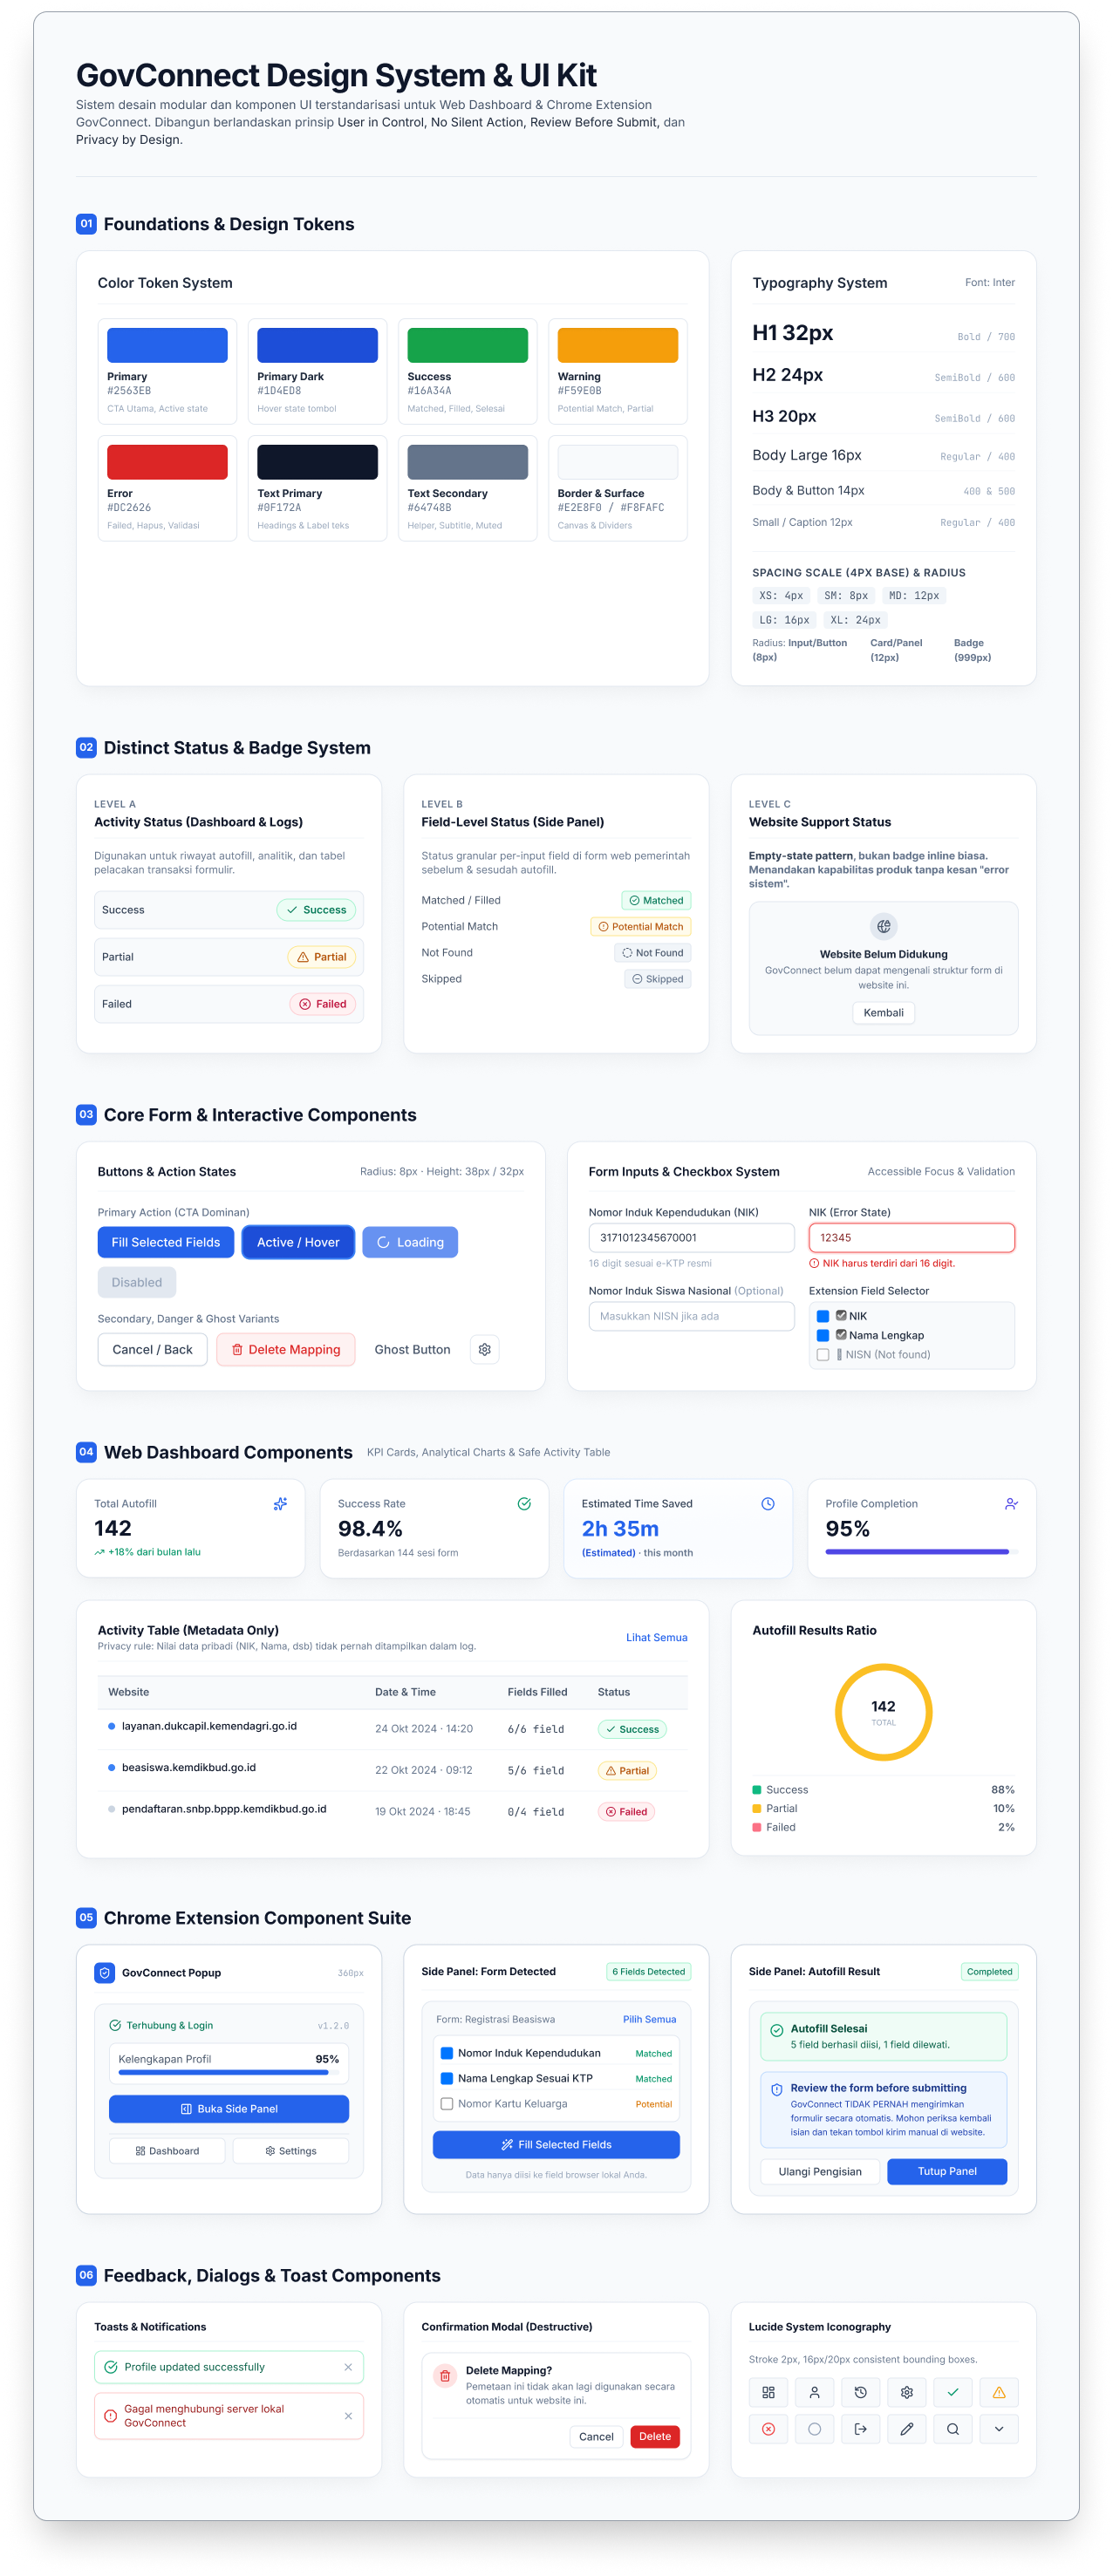
\includegraphics[width=0.8\textwidth, height=0.82\textheight, keepaspectratio]{designsystem.png}
\caption{Sistem Desain dan Komponen UI GovConnect.}
\label{fig:design_system}
\end{figure}

\clearpage
% ==========================================================
% SECTION IV: ARSITEKTUR SISTEM (ALUR & TECH STACK)
% ==========================================================
\section{Arsitektur Sistem (Alur \& Tech Stack)}

Arsitektur sistem GovConnect dirancang dengan memisahkan antarmuka interaksi pengguna (\textit{browser extension} dan \textit{web dashboard}) dari layanan backend (\textit{RESTful API} berbasis FastAPI dan basis data MySQL), sebagaimana ditampilkan pada Gambar~\ref{fig:arsitektur_sistem}.

\begin{figure}[!ht]
\centering
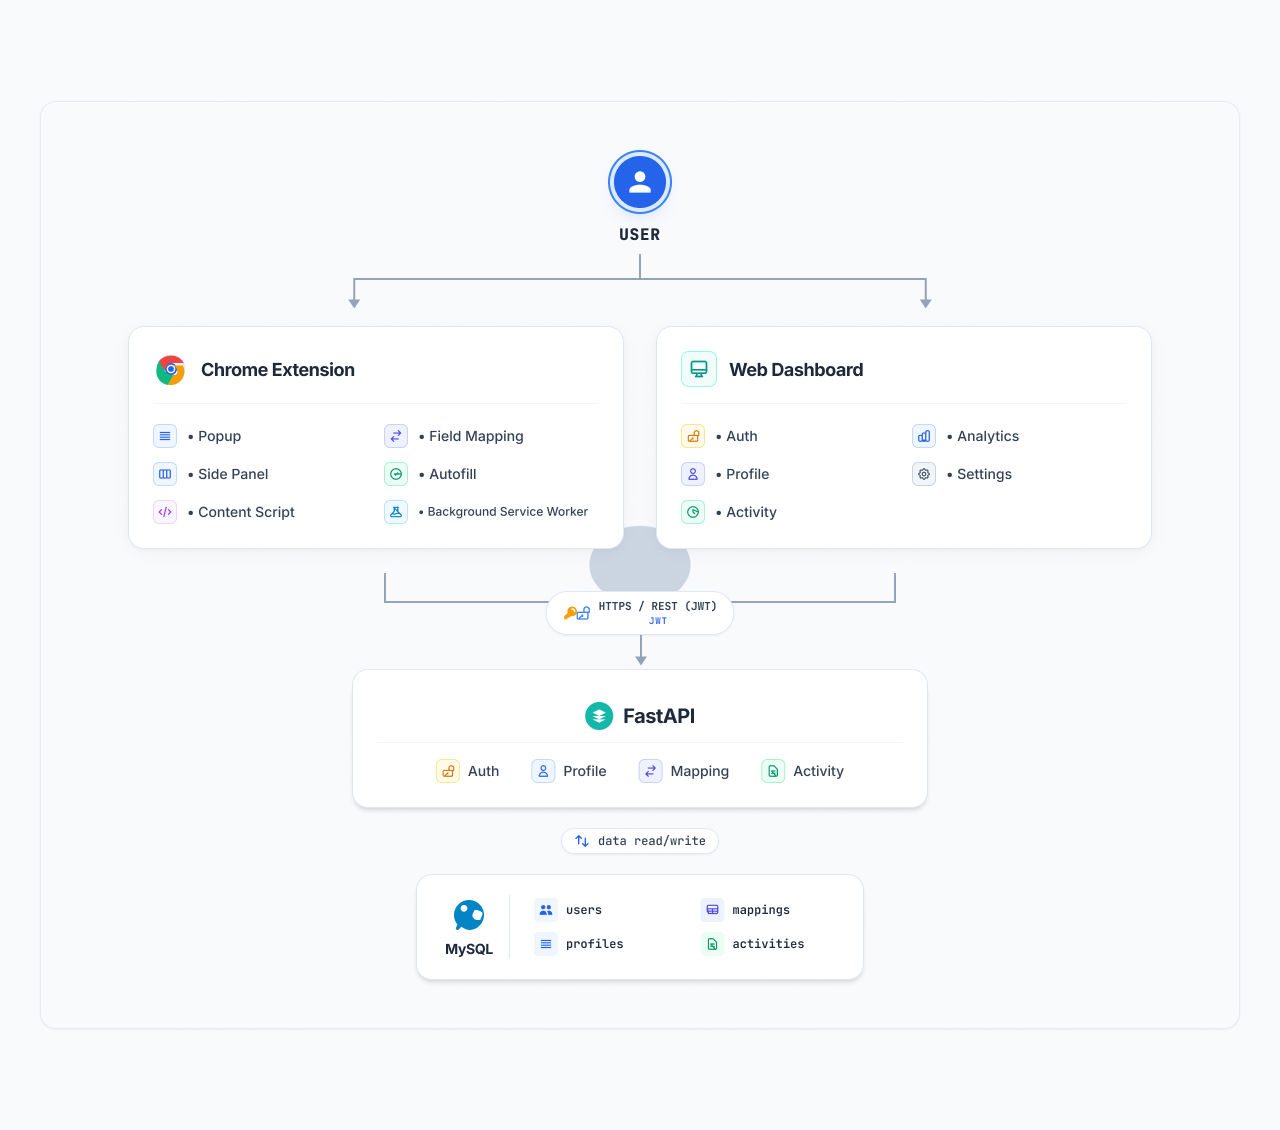
\includegraphics[width=0.75\textwidth]{Arsitektur Sistem.png}
\caption{Diagram Arsitektur Sistem GovConnect.}
\label{fig:arsitektur_sistem}
\end{figure}

Struktur relasi dan aliran data antarkomponen arsitektur sistem GovConnect didefinisikan secara deklaratif menggunakan diagram alur \textit{Mermaid} pada Listing~\ref{lst:mermaid_architecture}. Diagram ini menggambarkan batas segregasi tanggung jawab antara lingkungan pengguna (\textit{User Space}), lingkungan peramban web (\textit{Google Chrome Browser}), lapisan logika server (\textit{FastAPI Server}), dan lapisan persistensi data relasional (\textit{MySQL Database}).

\begin{lstlisting}[caption={Spesifikasi Diagram Arsitektur Sistem GovConnect (Mermaid)}, label={lst:mermaid_architecture}]
flowchart TB
    subgraph UserSpace["Lingkungan Pengguna & Browser"]
        User["Pengguna (End User)"]
        subgraph Browser["Google Chrome Browser"]
            Dashboard["Web Dashboard (React 18 + TS + Vite) :5173"]
            Extension["Browser Extension (Manifest V3 Vanilla JS)"]
        end
        User -->|Akses Dashboard| Dashboard
        User -->|Buka Form & Isi Data| Extension
    end

    subgraph BackendSpace["Lingkungan Backend (FastAPI Server :8000)"]
        Backend["FastAPI Application"]
        AuthModule["Auth Module (JWT HS256 + Bcrypt)"]
        APIRouter["Core API Router (/api/v1/...)"]
        ORM["SQLAlchemy ORM Layer"]
        Backend --> AuthModule
        Backend --> APIRouter
        AuthModule --> ORM
        APIRouter --> ORM
    end

    subgraph DatabaseSpace["Lingkungan Database"]
        DB[("MySQL 8.x Database (govconnect_db)")]
    end

    Dashboard -->|REST / HTTP + Bearer JWT| Backend
    Extension -->|REST / HTTP + Bearer JWT| Backend
    ORM -->|PyMySQL Connection Pool| DB
\end{lstlisting}

\subsection{Alur Pengguna (User Flow)}
Alur interaksi pengguna dengan sistem GovConnect terbagi menjadi dua alur kerja utama, yaitu proses \textit{Onboarding \& Profile Setup} (Gambar~\ref{fig:userflow_onboarding}) serta proses \textit{Autofill Flow} pada situs layanan publik (Gambar~\ref{fig:userflow_autofill}).

\begin{figure}[!ht]
\centering
\begin{minipage}[t]{0.42\textwidth}
\centering
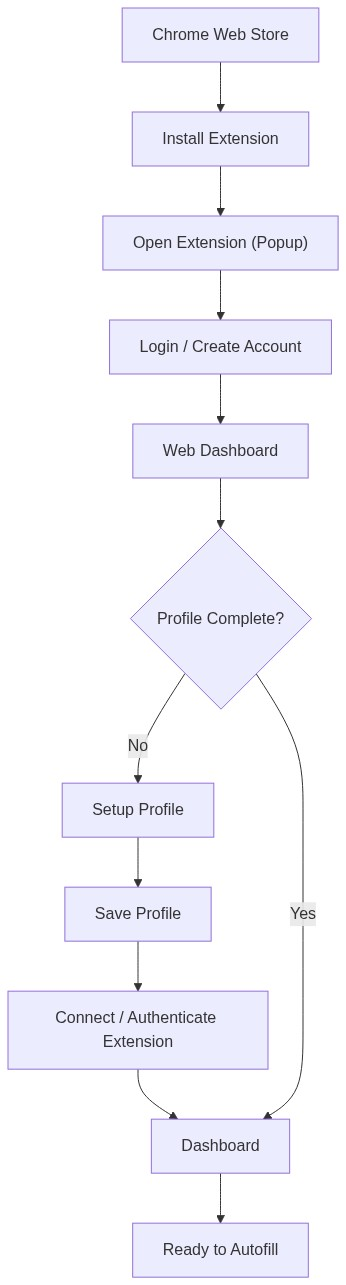
\includegraphics[height=0.65\textheight, keepaspectratio]{userflow_onboarding.png}
\caption{Alur \textit{Onboarding} \& Setup Profil.}
\label{fig:userflow_onboarding}
\end{minipage}
\hfill
\begin{minipage}[t]{0.54\textwidth}
\centering
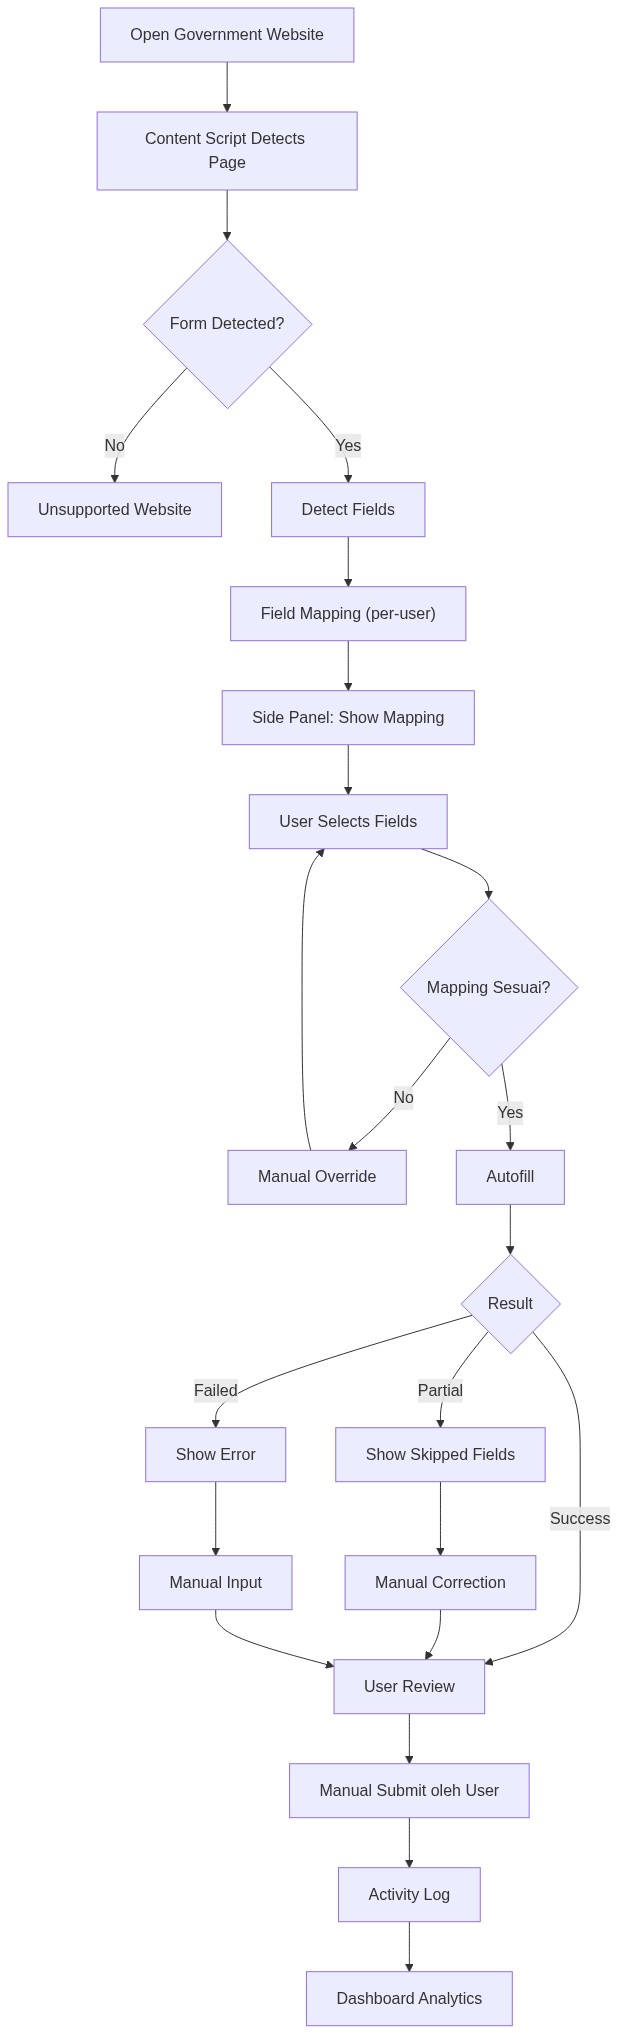
\includegraphics[height=0.65\textheight, keepaspectratio]{userflow_autofill.png}
\caption{Alur Pengisian Formulir (\textit{Autofill Flow}).}
\label{fig:userflow_autofill}
\end{minipage}
\end{figure}

\clearpage
% ==========================================================
% SECTION V: MOCKUP UI
% ==========================================================
\section{Mockup UI}

Perancangan antarmuka pengguna (\textit{User Interface}) GovConnect dibagi menjadi dua lingkungan operasional utama, yaitu \textit{Web Dashboard} untuk manajemen data pribadi dan analitik, serta \textit{Chrome Extension} (termasuk \textit{Side Panel}) untuk interaksi pengisian otomatis pada halaman formulir layanan publik.

\subsection{Antarmuka Web Dashboard}
Bagian \textit{Web Dashboard} memfasilitasi pengguna dalam memantau statistik aktivitas, memutakhirkan data identitas kependudukan, serta mengelola konfigurasi akun:

\begin{figure}[!ht]
\centering
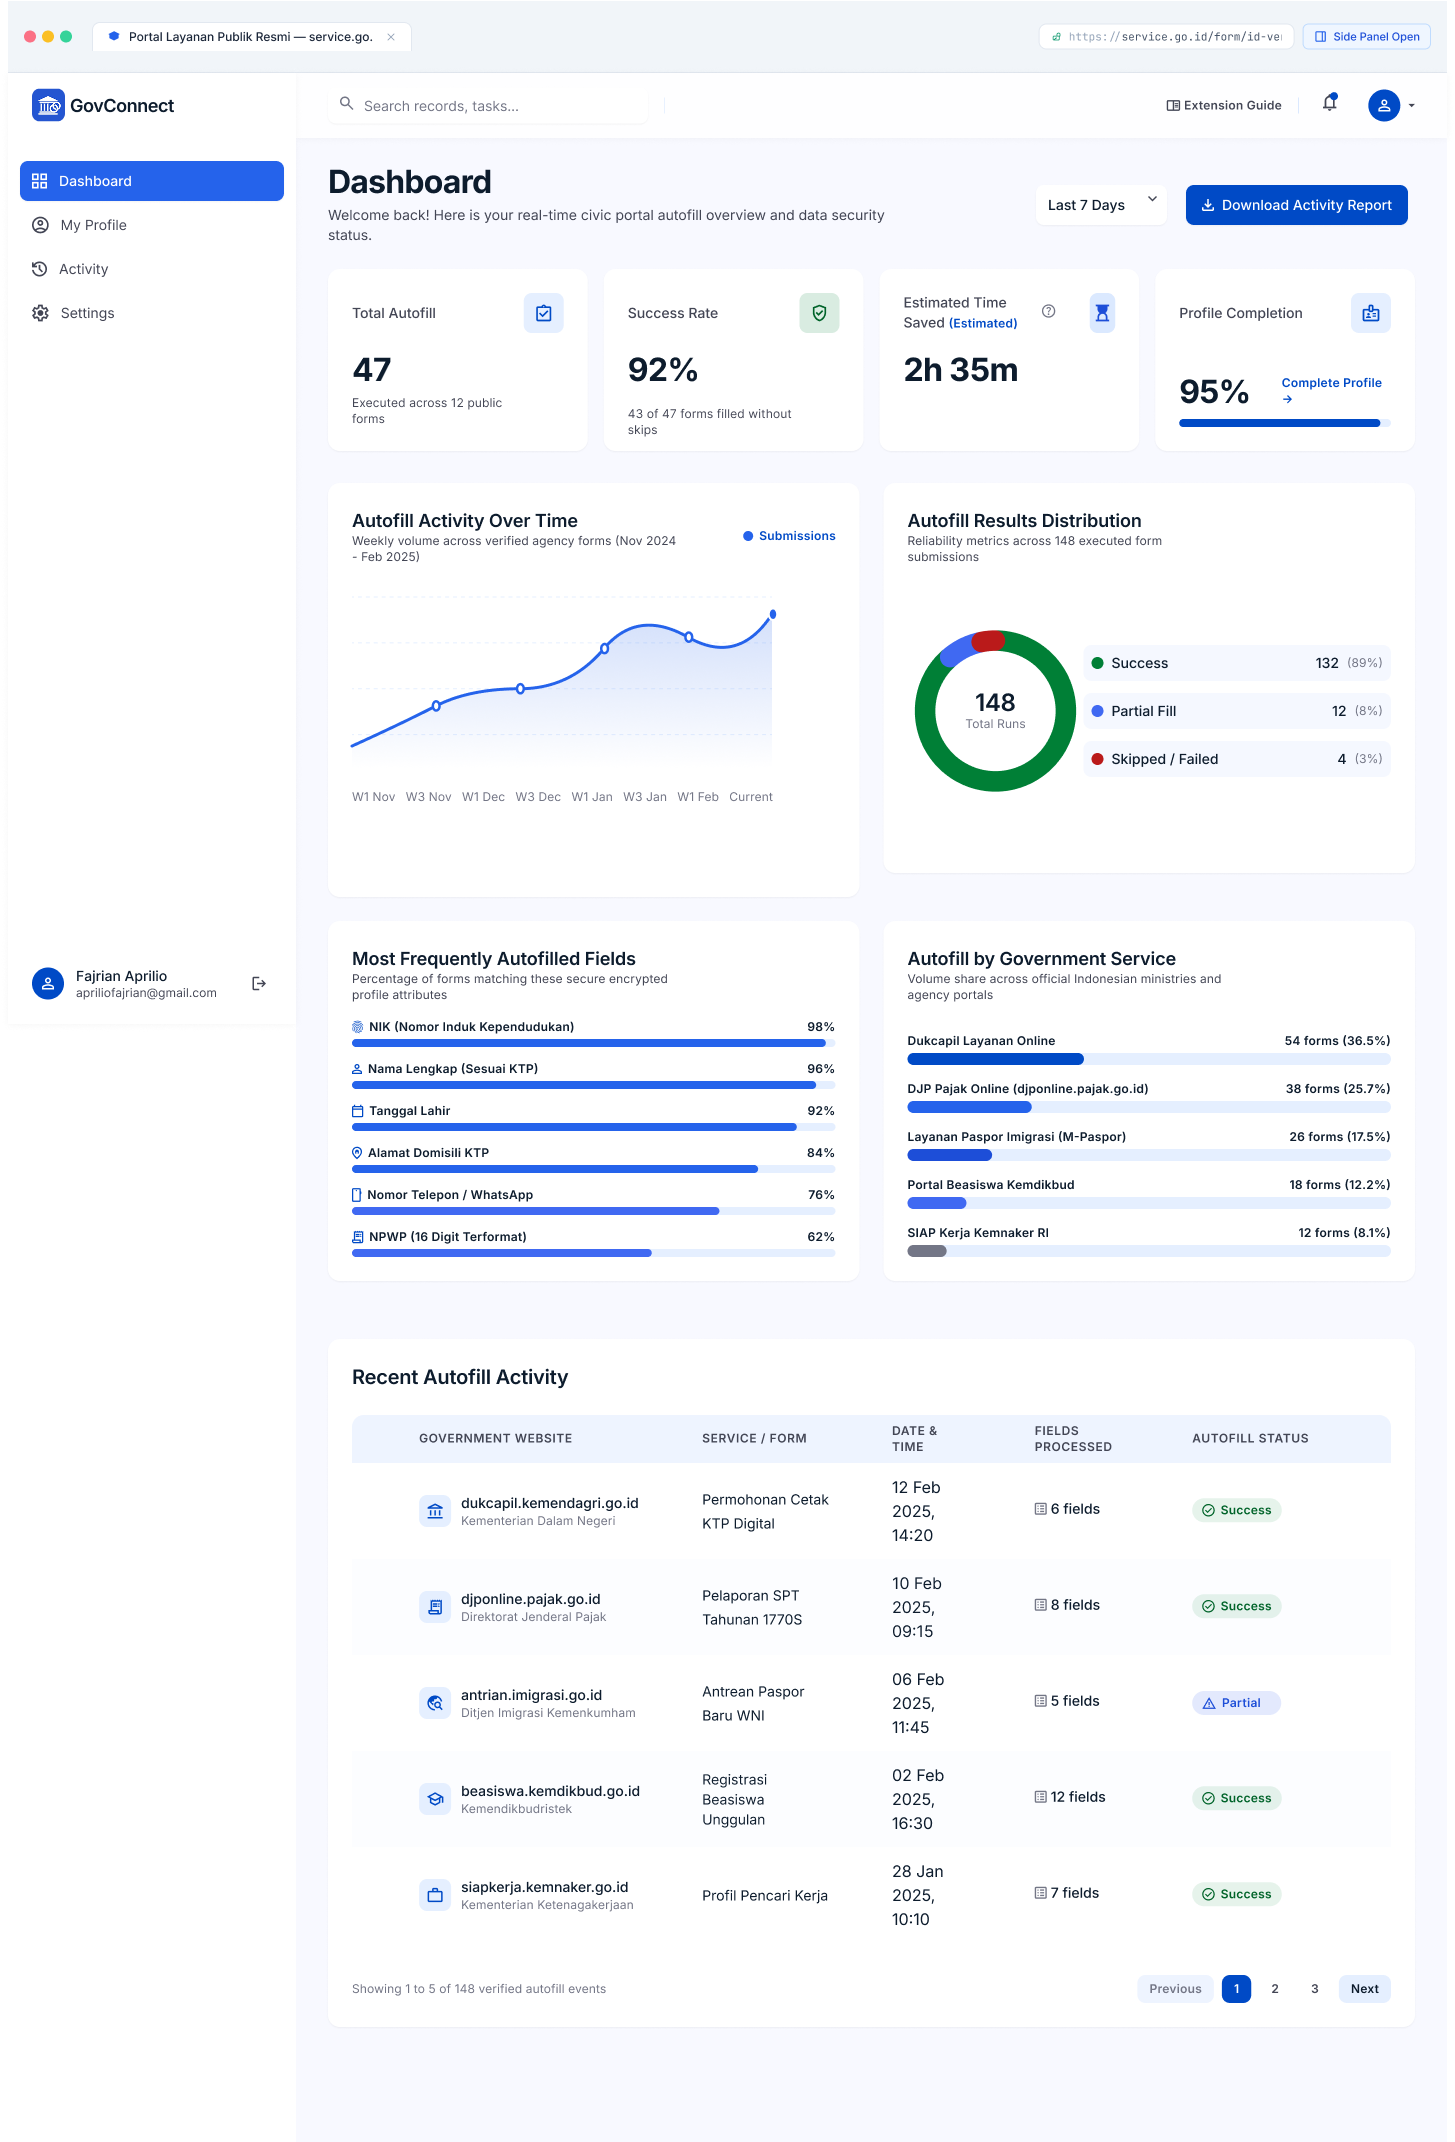
\includegraphics[width=0.65\textwidth, height=0.50\textheight, keepaspectratio]{Main Dashboard.png}
\caption{Antarmuka Halaman Utama (\textit{Main Dashboard}) GovConnect.}
\label{fig:mockup_dashboard}
\end{figure}

\begin{figure}[!ht]
\centering
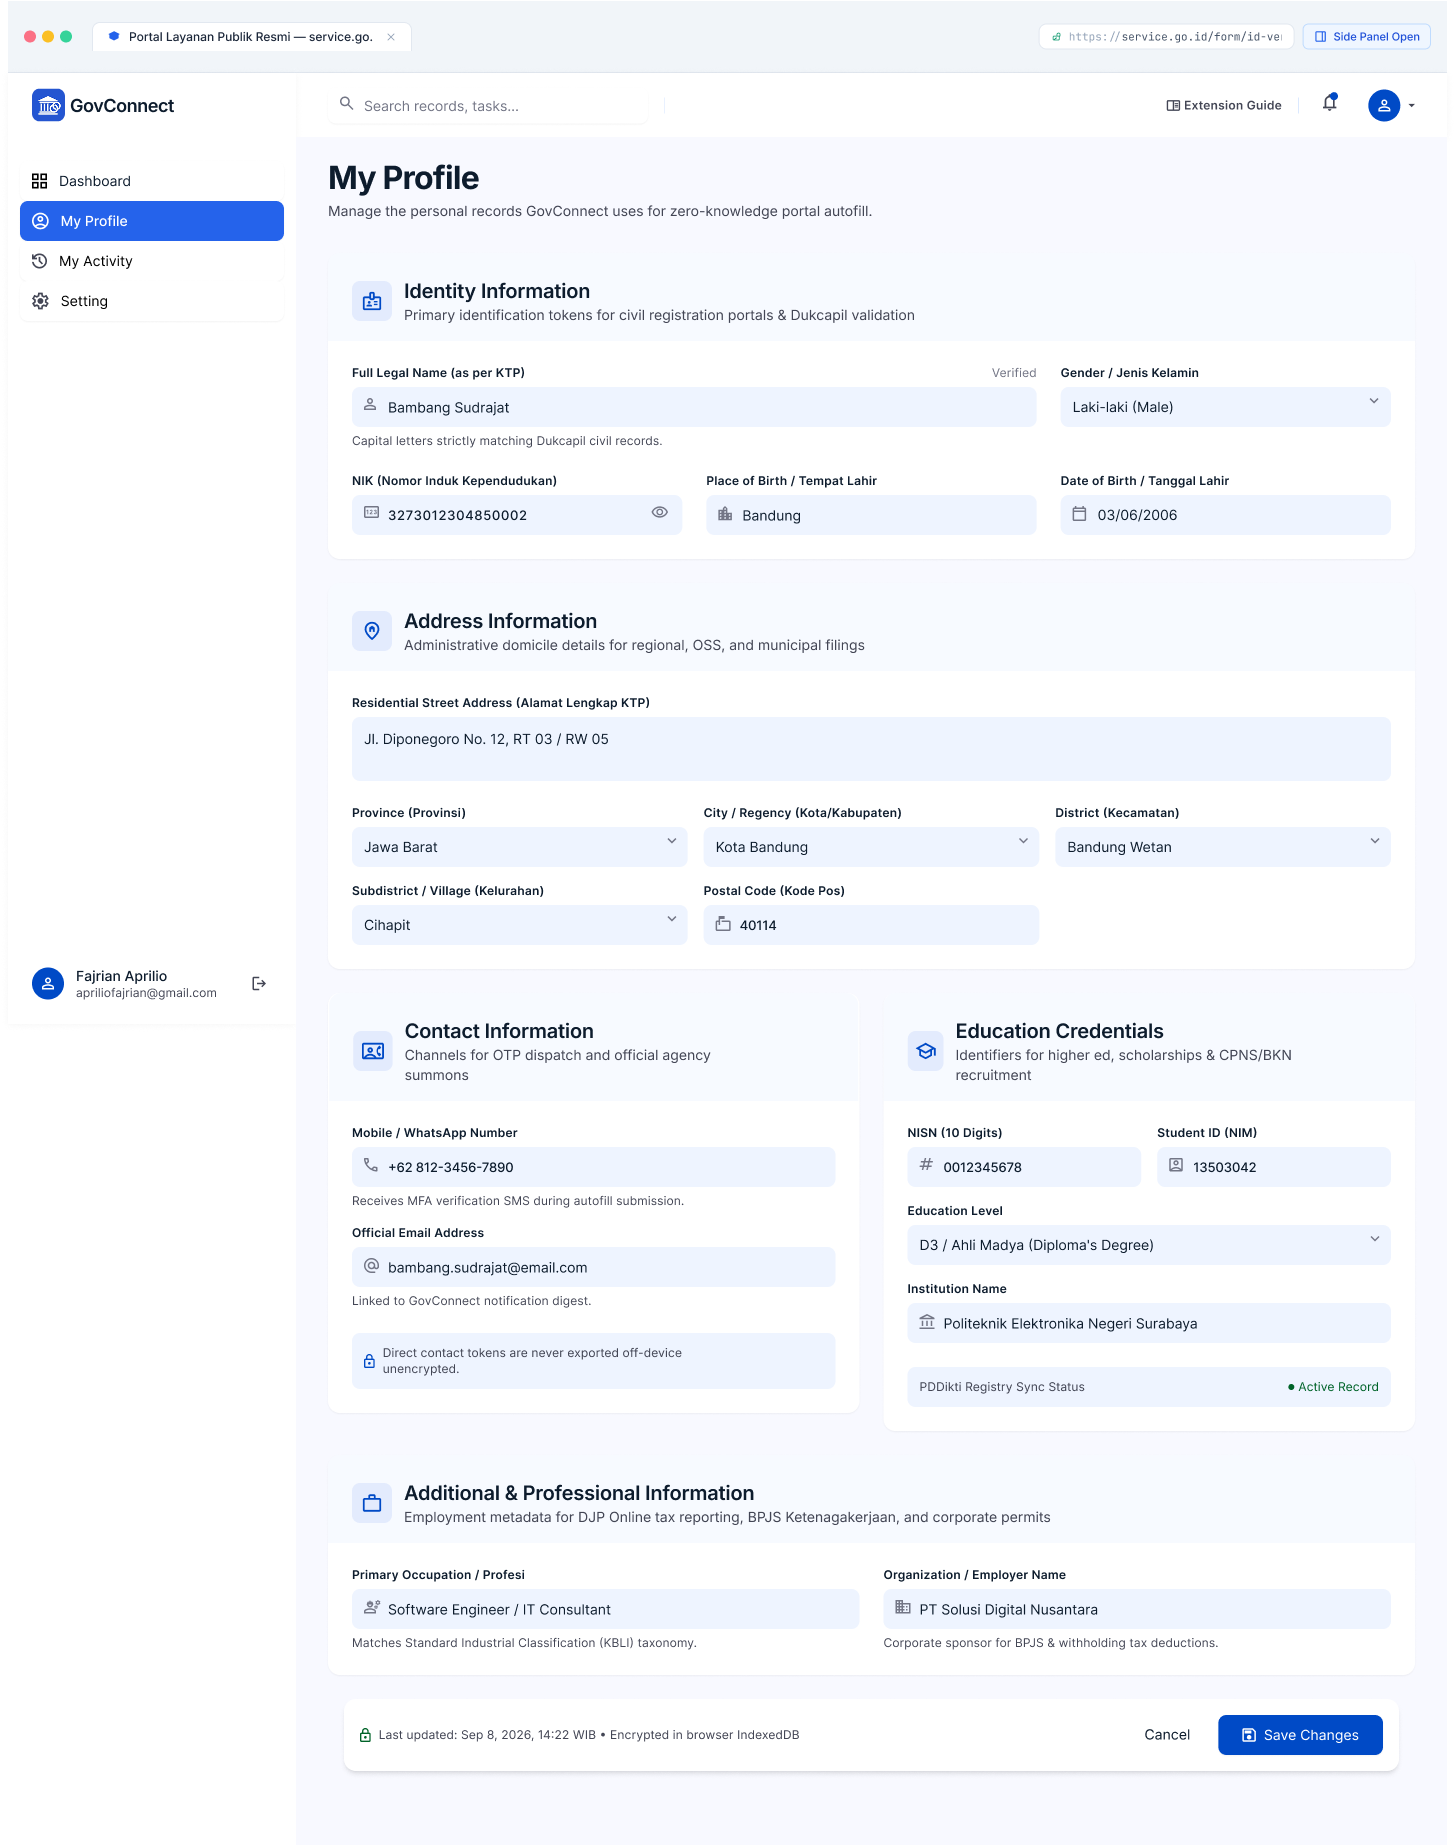
\includegraphics[width=0.65\textwidth, height=0.40\textheight, keepaspectratio]{My Profile.png}
\caption{Halaman Pengelolaan Data Profil Pengguna (\textit{My Profile}).}
\label{fig:mockup_profile}
\end{figure}

\begin{figure}[!ht]
\centering
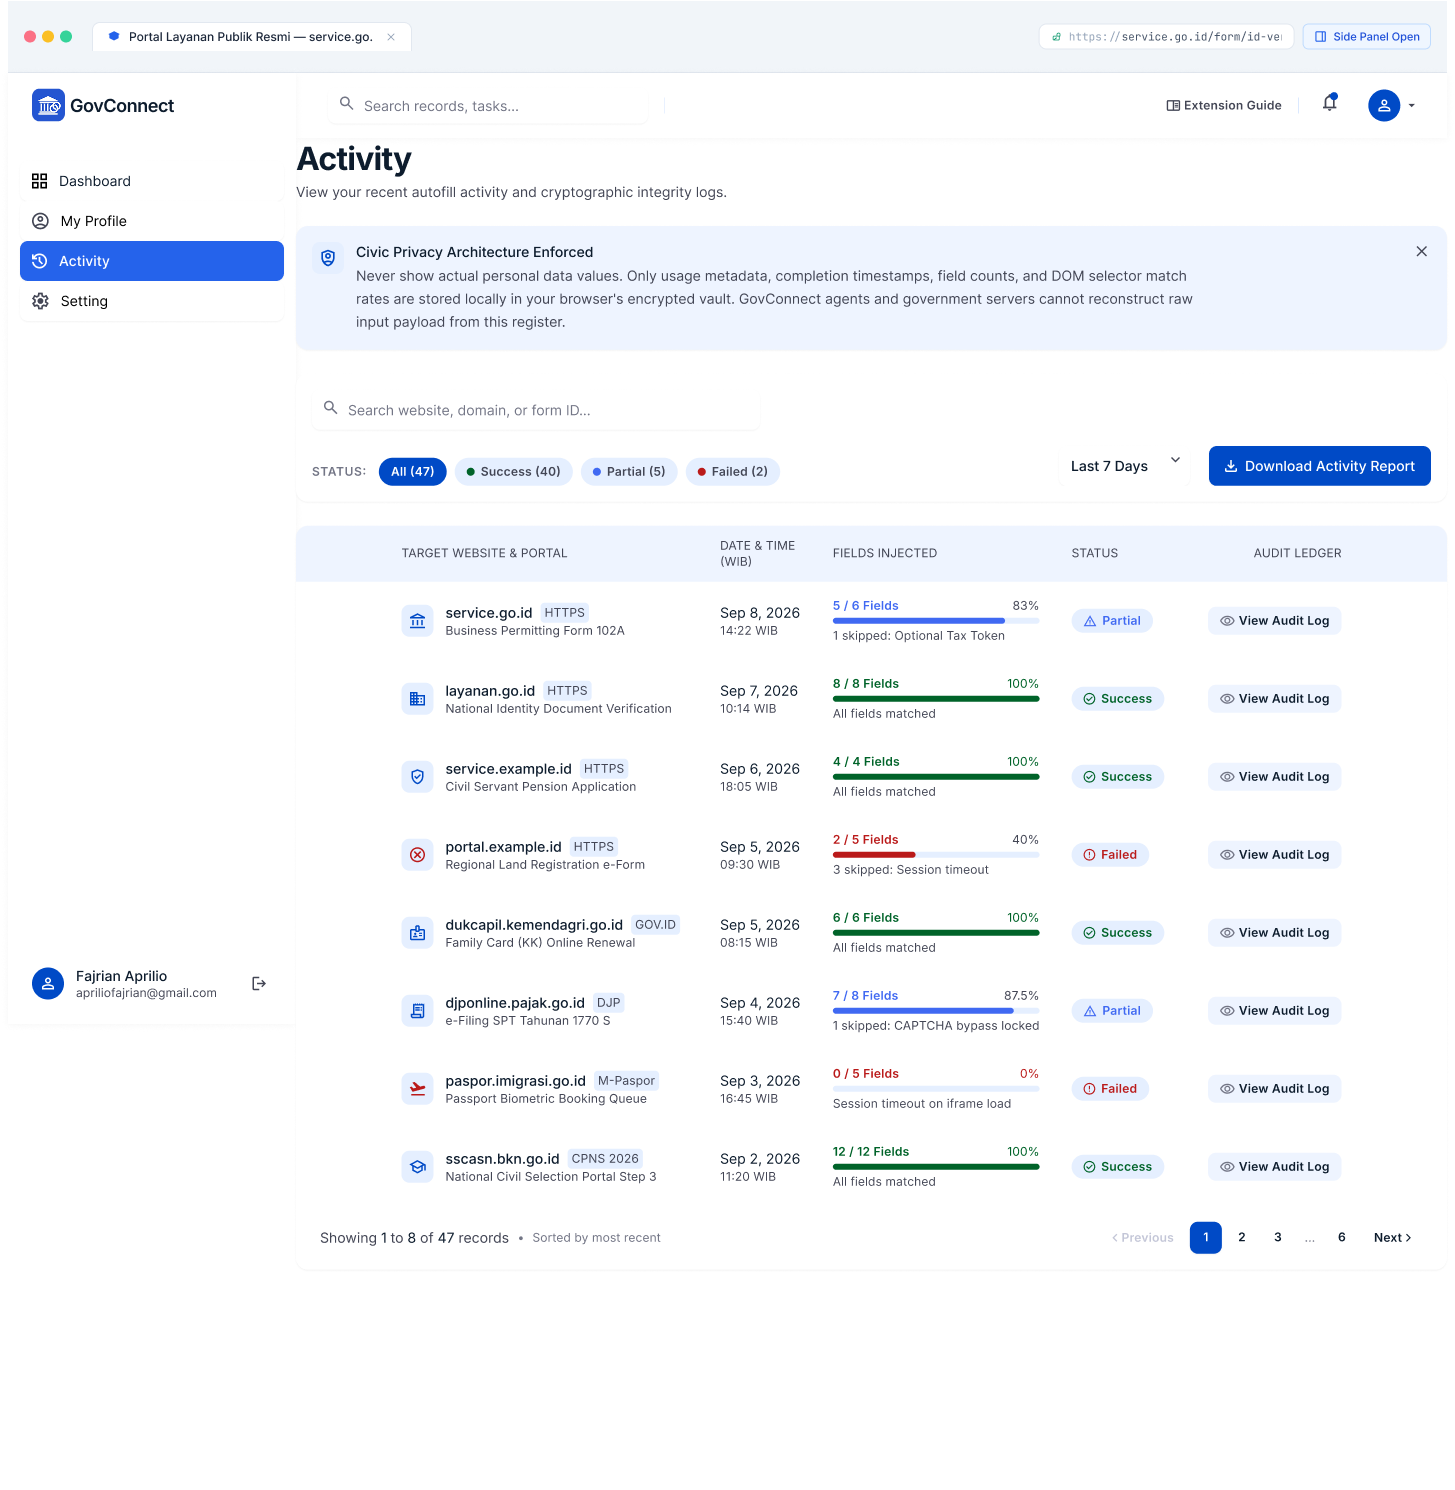
\includegraphics[width=0.65\textwidth, height=0.40\textheight, keepaspectratio]{Activity.png}
\caption{Halaman Riwayat Log Aktivitas Pengisian Formulir (\textit{Activity Log}).}
\label{fig:mockup_activity}
\end{figure}

\begin{figure}[!ht]
\centering
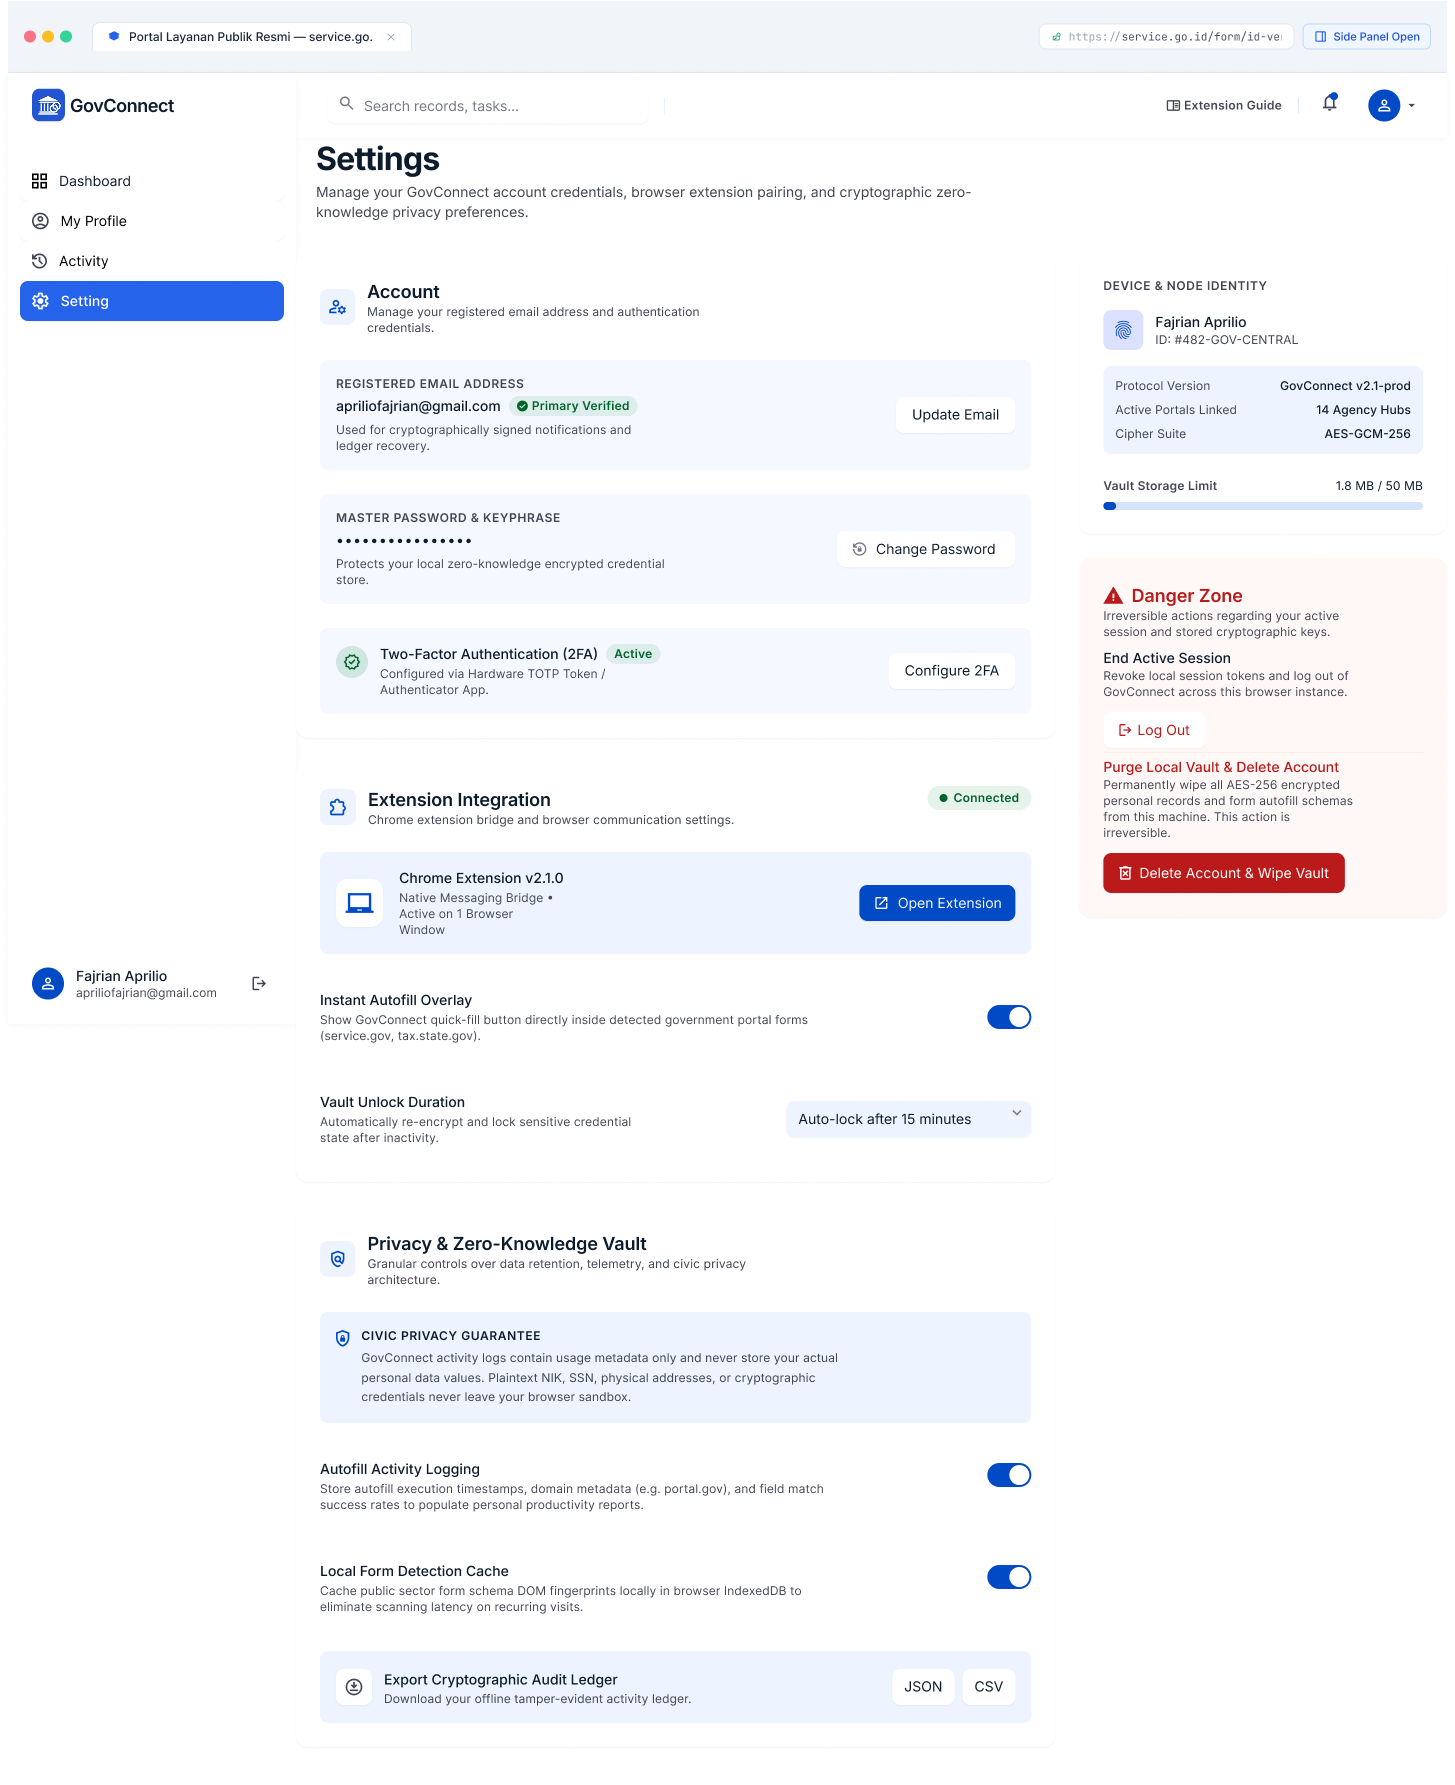
\includegraphics[width=0.65\textwidth, height=0.40\textheight, keepaspectratio]{Setting.png}
\caption{Halaman Pengaturan Akun dan Preferensi Sistem (\textit{Settings}).}
\label{fig:mockup_setting}
\end{figure}

\subsection{Antarmuka Chrome Extension \& Side Panel}
Bagian ekstensi peramban menyajikan interaksi langsung pada situs web target yang mencakup berbagai kondisi operasional:

\begin{figure}[!ht]
\centering
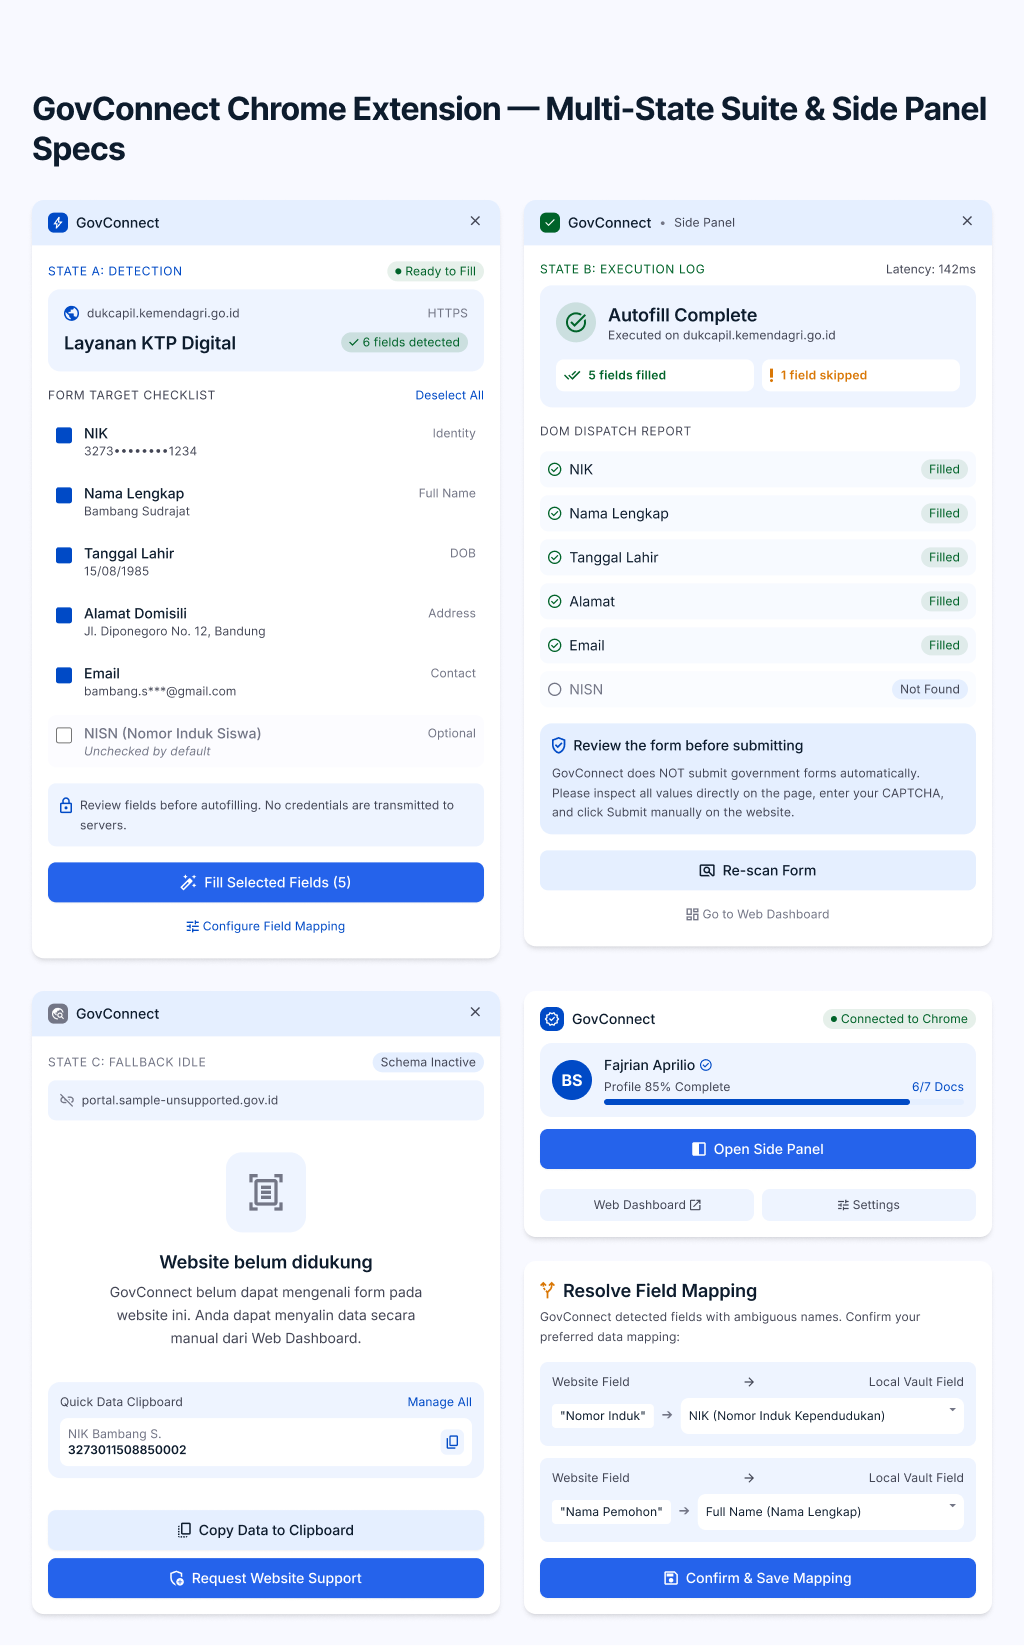
\includegraphics[width=0.45\textwidth, height=0.42\textheight, keepaspectratio]{Frontend Extension.png}
\caption{Tampilan Antarmuka \textit{Popup} Ekstensi Peramban GovConnect.}
\label{fig:mockup_extension}
\end{figure}

\begin{figure}[!ht]
\centering
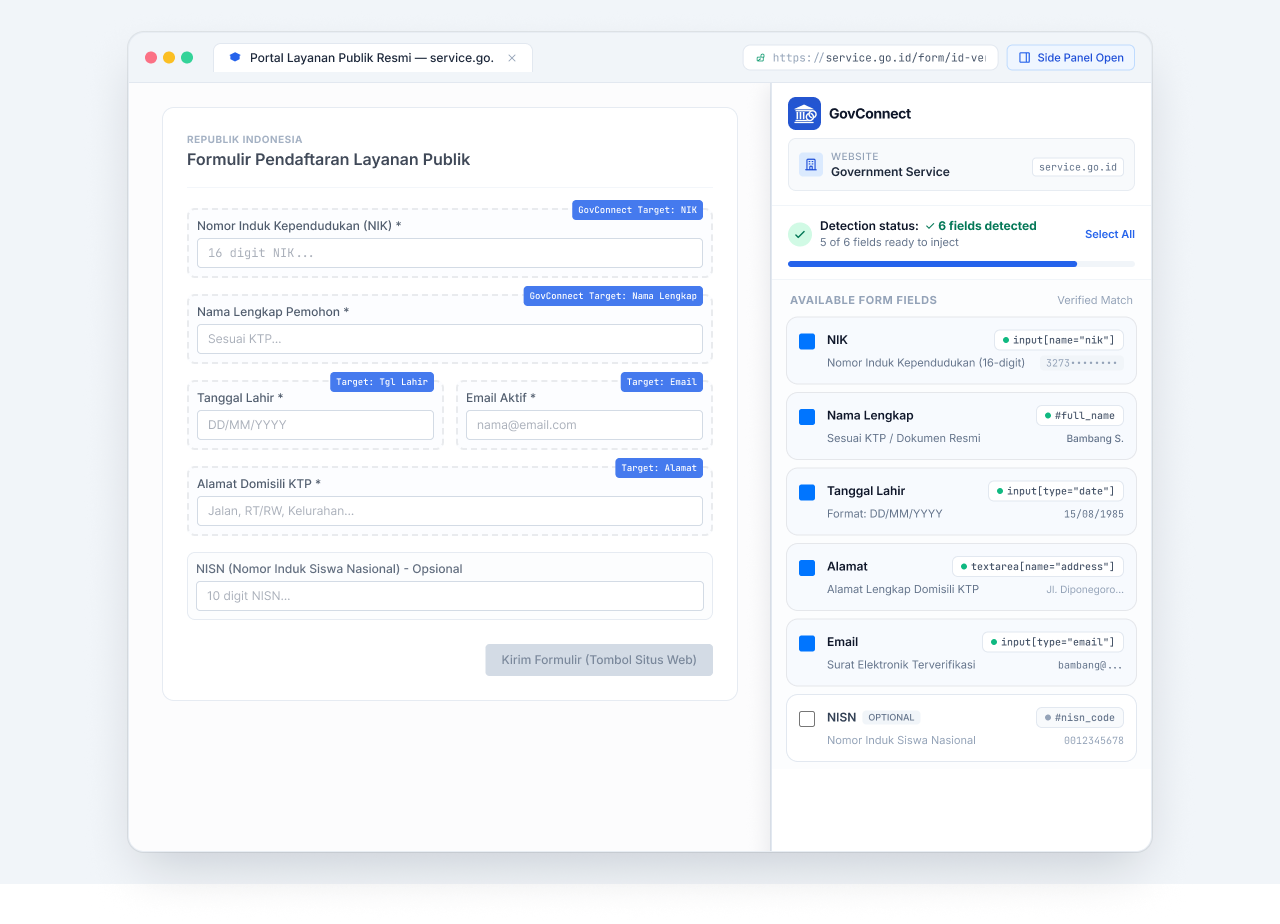
\includegraphics[width=0.65\textwidth, height=0.36\textheight, keepaspectratio]{Side Panel - Form Detected.png}
\caption{\textit{Side Panel}: Status Formulir Terdeteksi (\textit{Form Detected State}).}
\label{fig:mockup_sidepanel_detected}
\end{figure}

\begin{figure}[!ht]
\centering
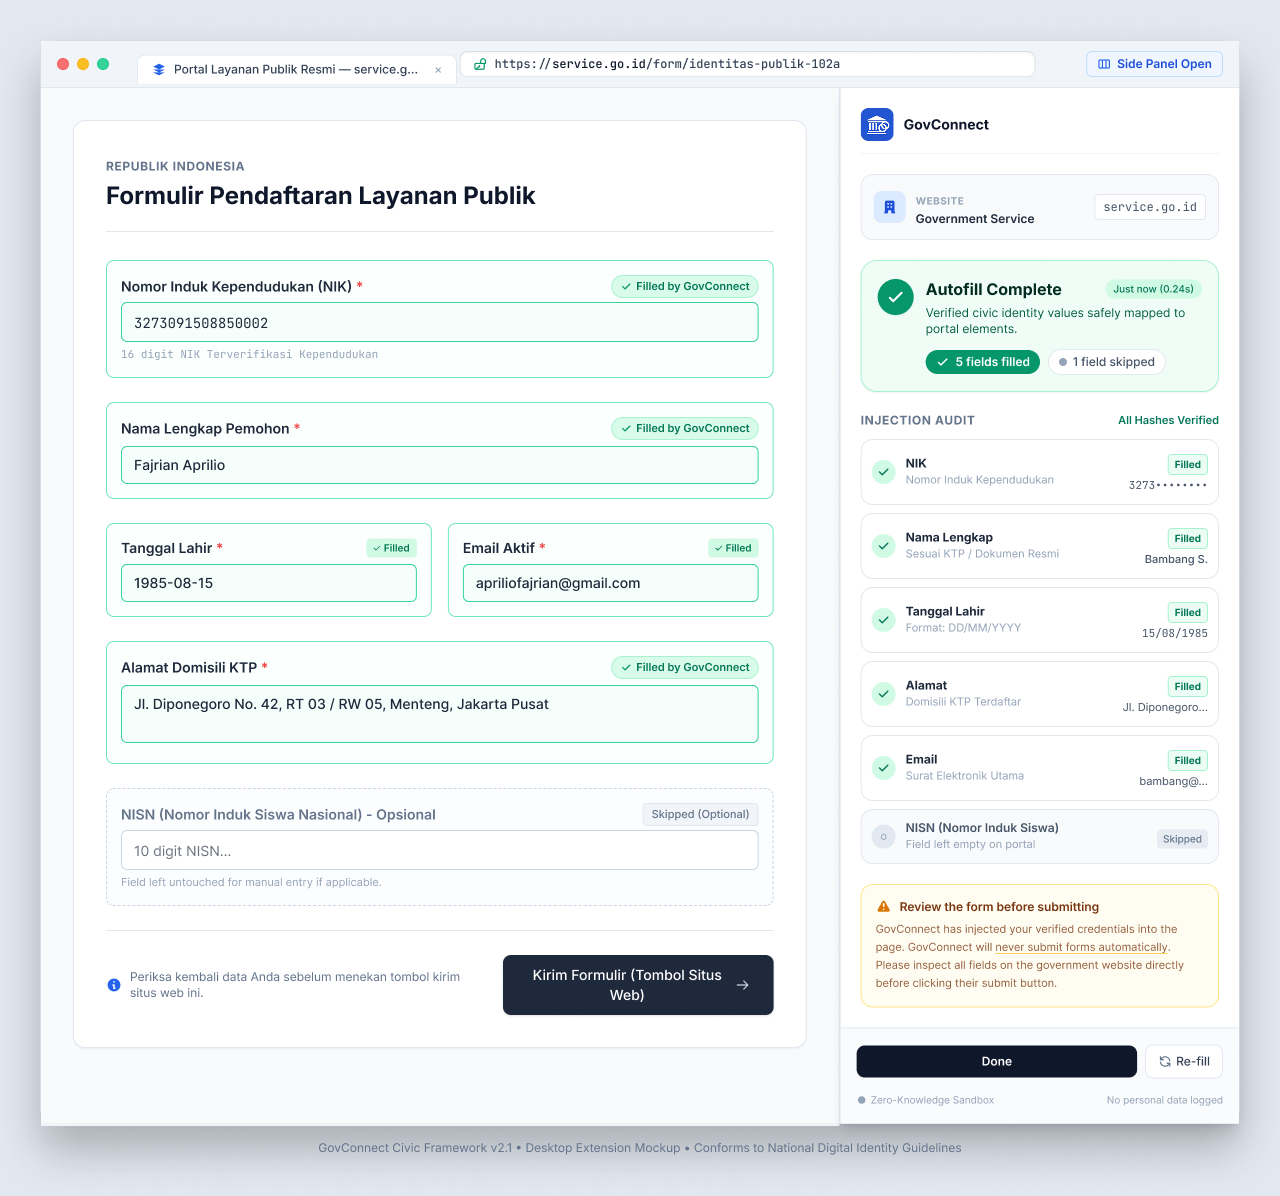
\includegraphics[width=0.65\textwidth, height=0.36\textheight, keepaspectratio]{Side Panel - Autofill Result.png}
\caption{\textit{Side Panel}: Rangkuman Hasil Pengisian (\textit{Autofill Result State}).}
\label{fig:mockup_sidepanel_result}
\end{figure}

\begin{figure}[!ht]
\centering
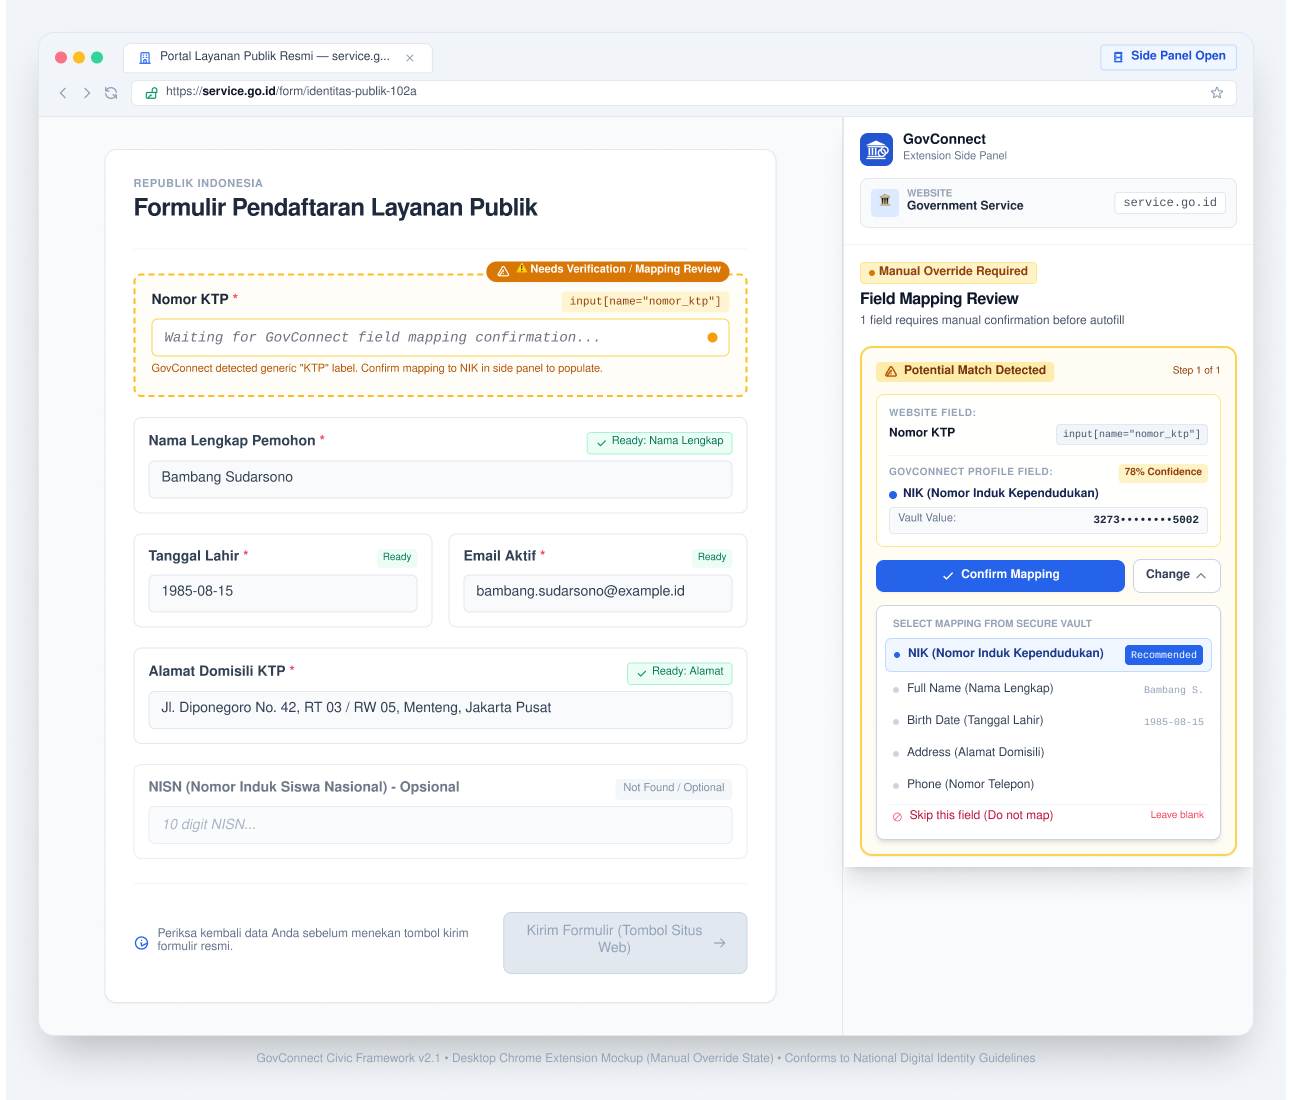
\includegraphics[width=0.65\textwidth, height=0.36\textheight, keepaspectratio]{Side Panel - Manual Override.png}
\caption{\textit{Side Panel}: Pemetaan Manual Field (\textit{Manual Override State}).}
\label{fig:mockup_sidepanel_override}
\end{figure}

\begin{figure}[!ht]
\centering
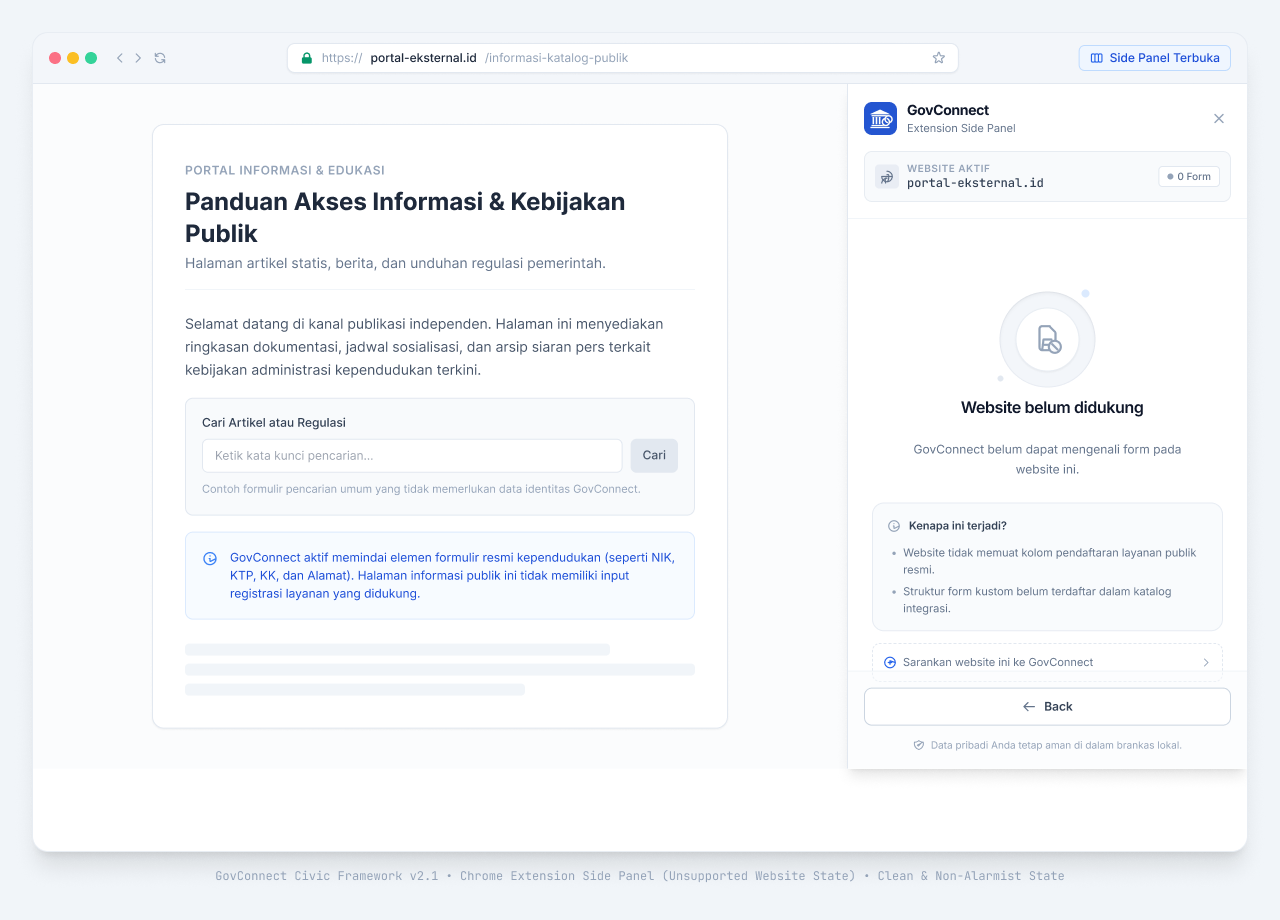
\includegraphics[width=0.65\textwidth, height=0.36\textheight, keepaspectratio]{Side Panel - Unsupported Website.png}
\caption{\textit{Side Panel}: Situs Web Belum Didukung (\textit{Unsupported Website State}).}
\label{fig:mockup_sidepanel_unsupported}
\end{figure}

\end{document}
\end{lstlisting}

\clearpage
% ==========================================================
% SECTION III: DESIGN SYSTEM
% ==========================================================
\section{Design System}

Perancangan visual dan komponen antarmuka GovConnect mengacu pada sistem desain terpadu yang mencakup token warna, tipografi, sistem status, serta komponen UI modular untuk \textit{web dashboard} dan ekstensi peramban, sebagaimana diilustrasikan pada Gambar~\ref{fig:design_system}.

\begin{figure}[htbp]
\centering
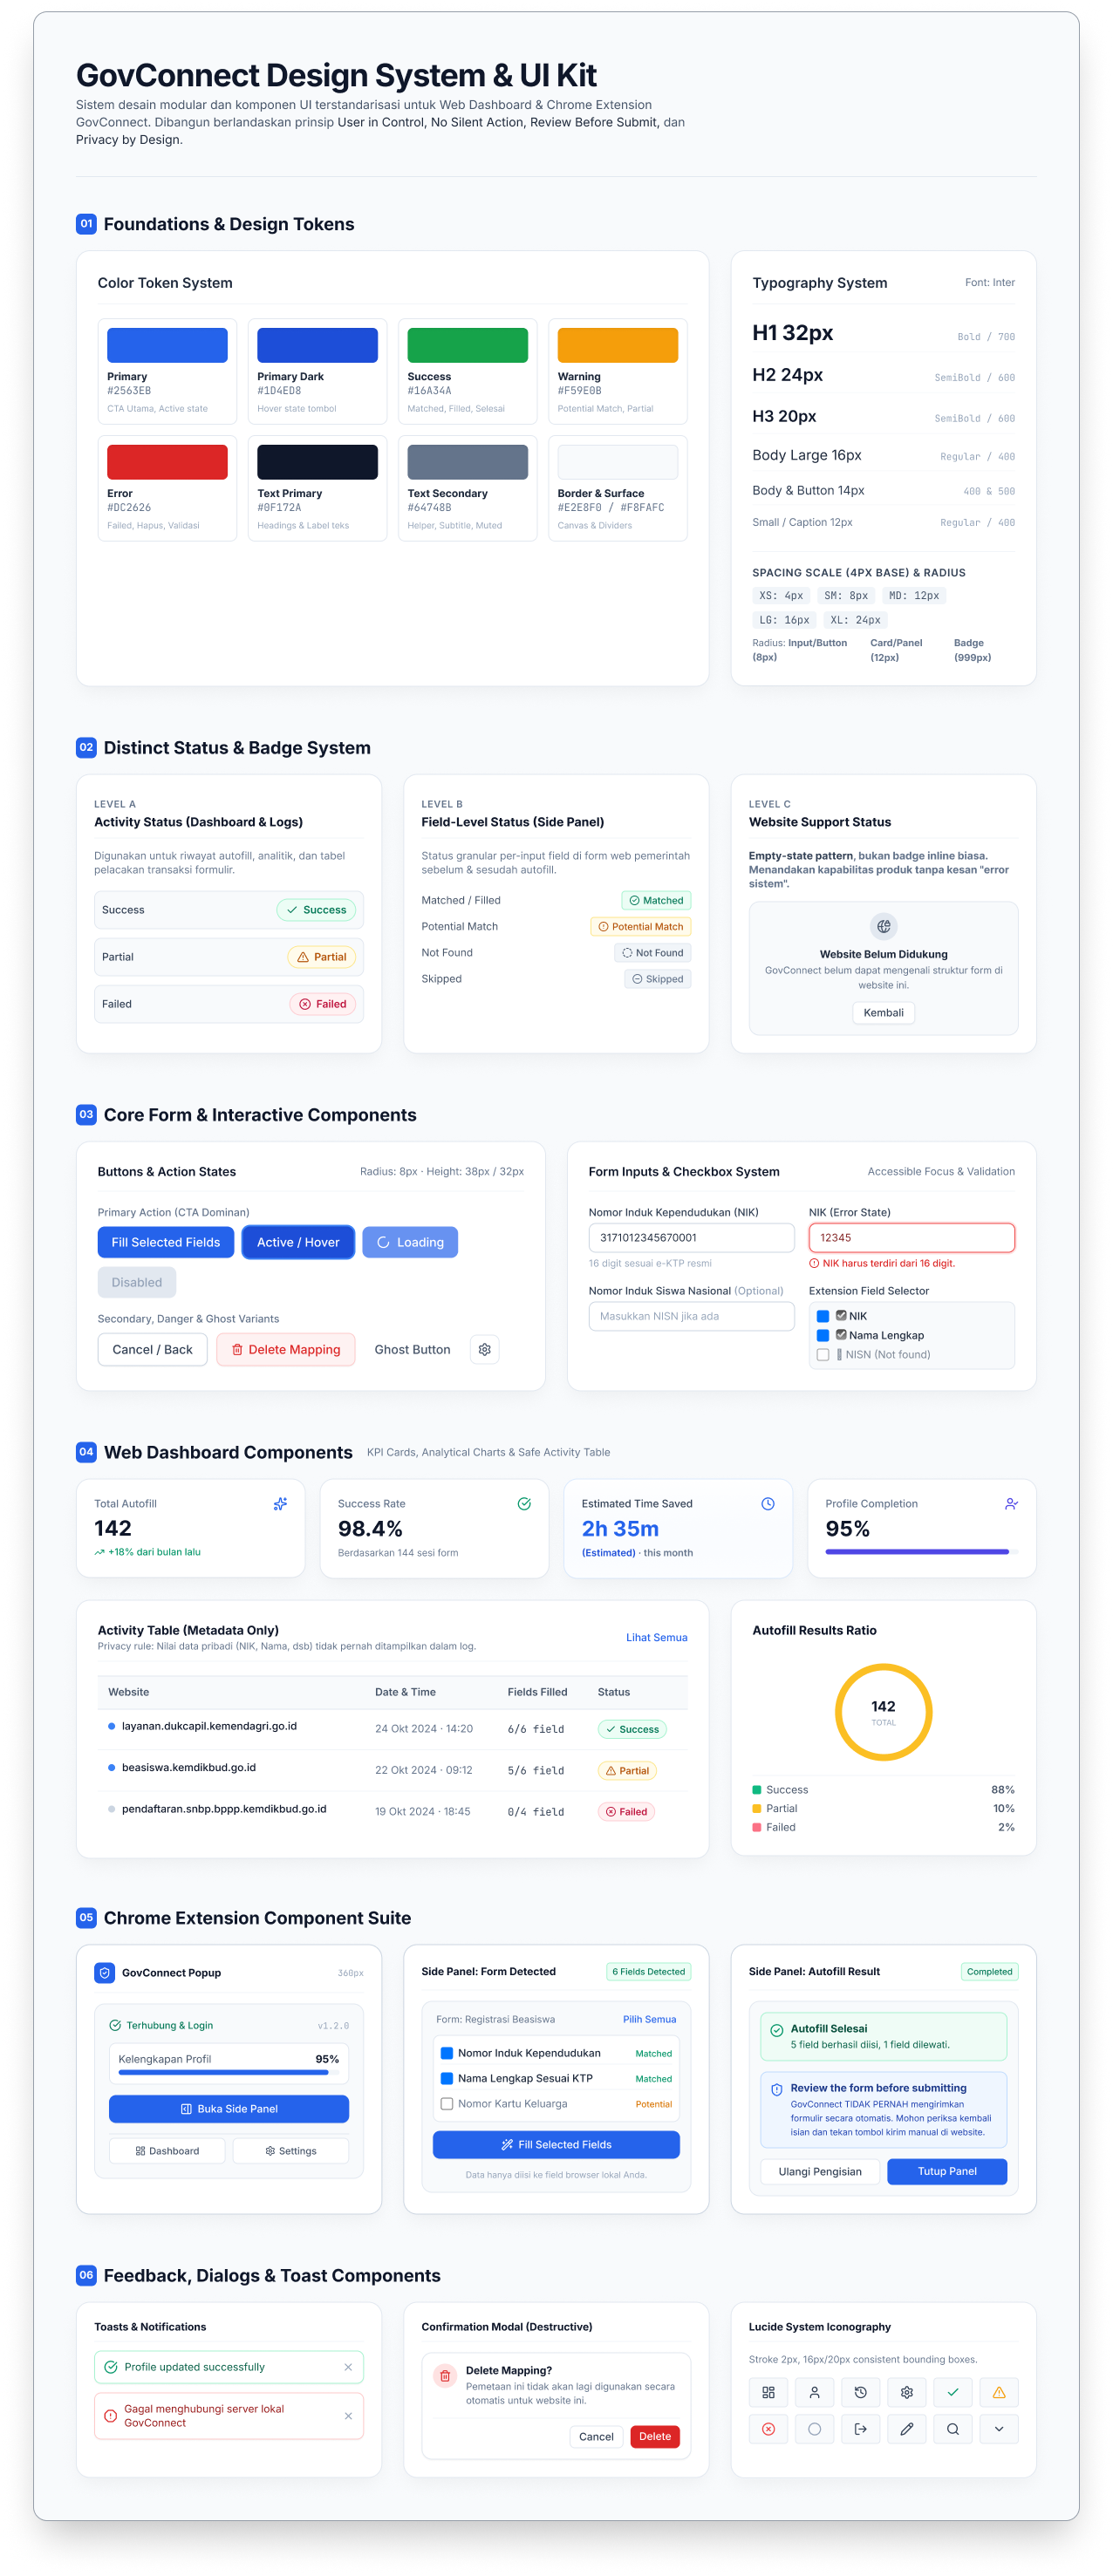
\includegraphics[width=0.8\textwidth, height=0.82\textheight, keepaspectratio]{designsystem.png}
\caption{Sistem Desain dan Komponen UI GovConnect.}
\label{fig:design_system}
\end{figure}

% Silakan isi source code LaTeX tambahan untuk bagian Design System di sini.


\clearpage
% ==========================================================
% SECTION IV: ARSITEKTUR SISTEM (ALUR & TECH STACK)
% ==========================================================
\section{Arsitektur Sistem (Alur \& Tech Stack)}

Arsitektur sistem GovConnect dirancang dengan memisahkan antarmuka interaksi pengguna (\textit{browser extension} dan \textit{web dashboard}) dari layanan backend (\textit{RESTful API} berbasis FastAPI dan basis data MySQL), sebagaimana ditampilkan pada Gambar~\ref{fig:arsitektur_sistem}.

\begin{figure}[!ht]
\centering
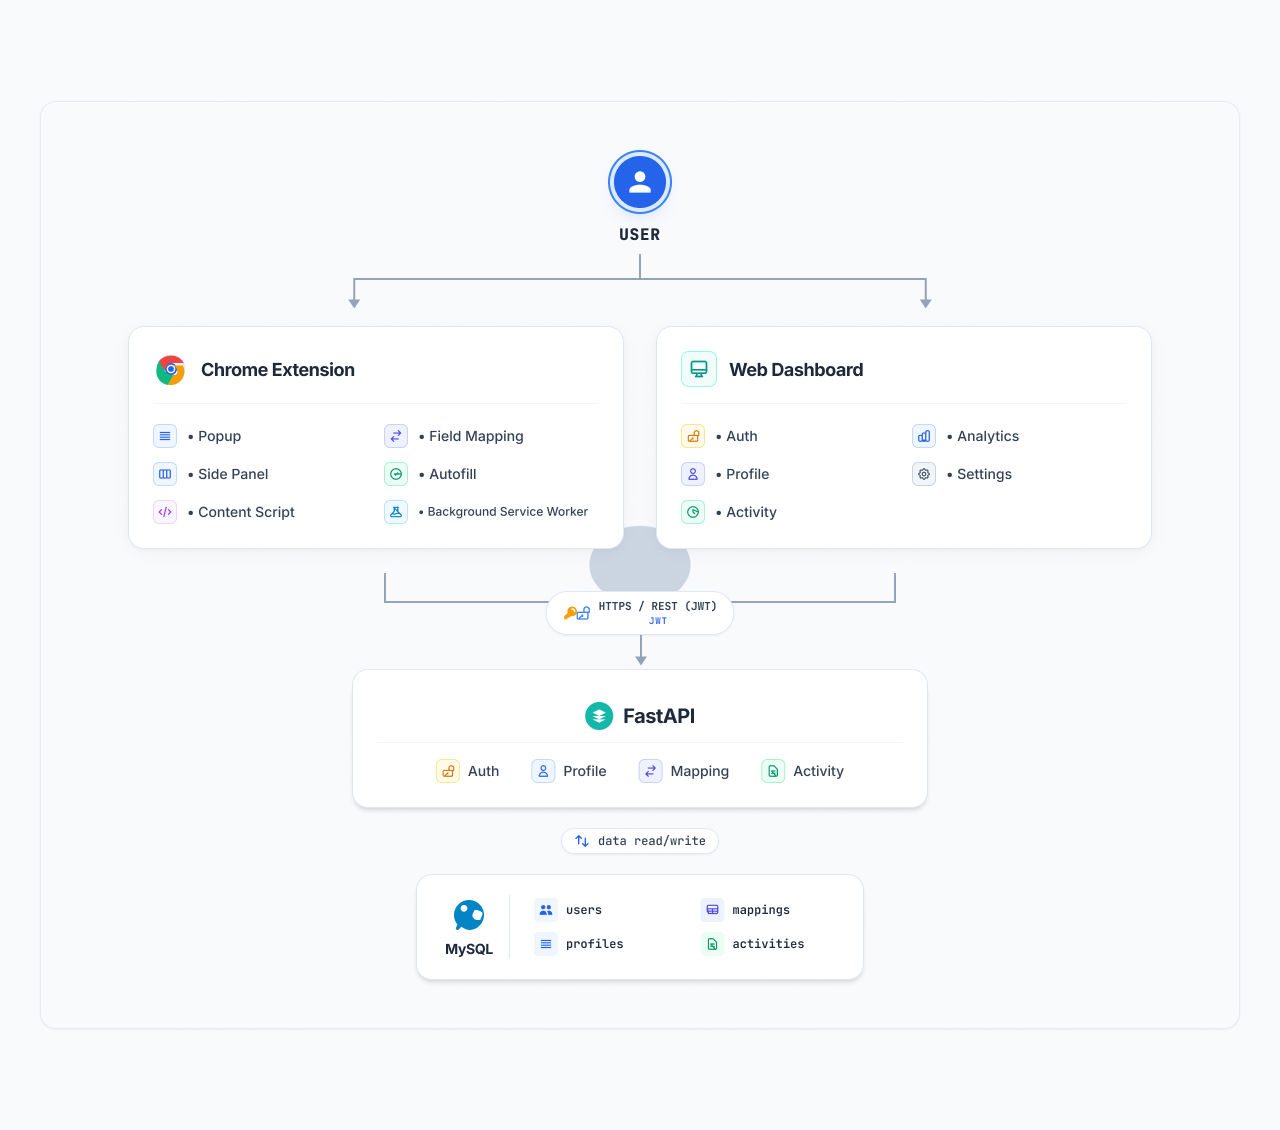
\includegraphics[width=0.75\textwidth]{Arsitektur Sistem.png}
\caption{Diagram Arsitektur Sistem GovConnect.}
\label{fig:arsitektur_sistem}
\end{figure}

Struktur relasi dan aliran data antarkomponen arsitektur sistem GovConnect didefinisikan secara deklaratif menggunakan diagram alur \textit{Mermaid} pada Listing~\ref{lst:mermaid_architecture}. Diagram ini menggambarkan batas segregasi tanggung jawab antara lingkungan pengguna (\textit{User Space}), lingkungan peramban web (\textit{Google Chrome Browser}), lapisan logika server (\textit{FastAPI Server}), dan lapisan persistensi data relasional (\textit{MySQL Database}).

\begin{lstlisting}[caption={Spesifikasi Diagram Arsitektur Sistem GovConnect (Mermaid)}, label={lst:mermaid_architecture}]
flowchart TB
    subgraph UserSpace["Lingkungan Pengguna & Browser"]
        User["Pengguna (End User)"]
        subgraph Browser["Google Chrome Browser"]
            Dashboard["Web Dashboard (React 18 + TS + Vite) :5173"]
            Extension["Browser Extension (Manifest V3 Vanilla JS)"]
        end
        User -->|Akses Dashboard| Dashboard
        User -->|Buka Form & Isi Data| Extension
    end

    subgraph BackendSpace["Lingkungan Backend (FastAPI Server :8000)"]
        Backend["FastAPI Application"]
        AuthModule["Auth Module (JWT HS256 + Bcrypt)"]
        APIRouter["Core API Router (/api/v1/...)"]
        ORM["SQLAlchemy ORM Layer"]
        Backend --> AuthModule
        Backend --> APIRouter
        AuthModule --> ORM
        APIRouter --> ORM
    end

    subgraph DatabaseSpace["Lingkungan Database"]
        DB[("MySQL 8.x Database (govconnect_db)")]
    end

    Dashboard -->|REST / HTTP + Bearer JWT| Backend
    Extension -->|REST / HTTP + Bearer JWT| Backend
    ORM -->|PyMySQL Connection Pool| DB
\end{lstlisting}

\subsection{Alur Pengguna (User Flow)}
Alur interaksi pengguna dengan sistem GovConnect terbagi menjadi dua alur kerja utama, yaitu proses \textit{Onboarding \& Profile Setup} (Gambar~\ref{fig:userflow_onboarding}) serta proses \textit{Autofill Flow} pada situs layanan publik (Gambar~\ref{fig:userflow_autofill}).

\begin{figure}[!ht]
\centering
\begin{minipage}[t]{0.42\textwidth}
\centering
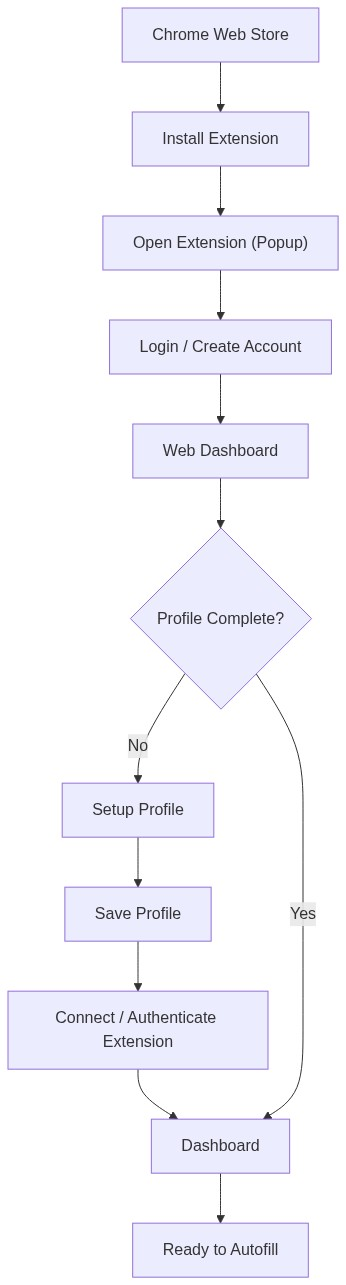
\includegraphics[height=0.65\textheight, keepaspectratio]{userflow_onboarding.png}
\caption{Alur \textit{Onboarding} \& Setup Profil.}
\label{fig:userflow_onboarding}
\end{minipage}
\hfill
\begin{minipage}[t]{0.54\textwidth}
\centering
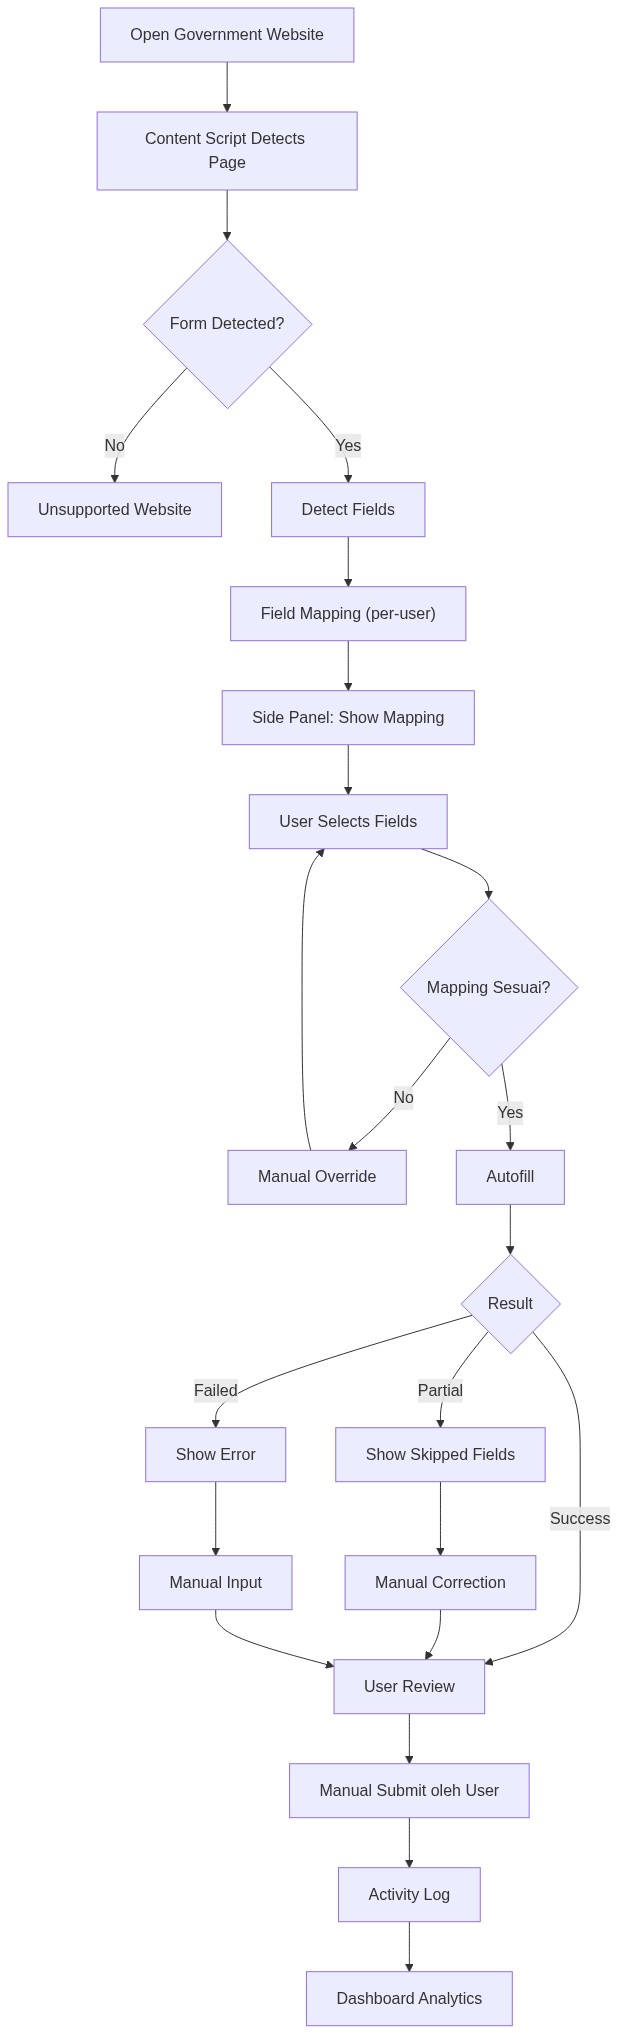
\includegraphics[height=0.65\textheight, keepaspectratio]{userflow_autofill.png}
\caption{Alur Pengisian Formulir (\textit{Autofill Flow}).}
\label{fig:userflow_autofill}
\end{minipage}
\end{figure}


\clearpage
% ==========================================================
% SECTION V: MOCKUP UI
% ==========================================================
\section{Mockup UI}

Perancangan antarmuka pengguna (\textit{User Interface}) GovConnect dibagi menjadi dua lingkungan operasional utama, yaitu \textit{Web Dashboard} untuk manajemen data pribadi dan analitik, serta \textit{Chrome Extension} (termasuk \textit{Side Panel}) untuk interaksi pengisian otomatis pada halaman formulir layanan publik.

\subsection{Antarmuka Web Dashboard}
Bagian \textit{Web Dashboard} memfasilitasi pengguna dalam memantau statistik aktivitas, memutakhirkan data identitas kependudukan, serta mengelola konfigurasi akun:

\begin{figure}[!ht]
\centering
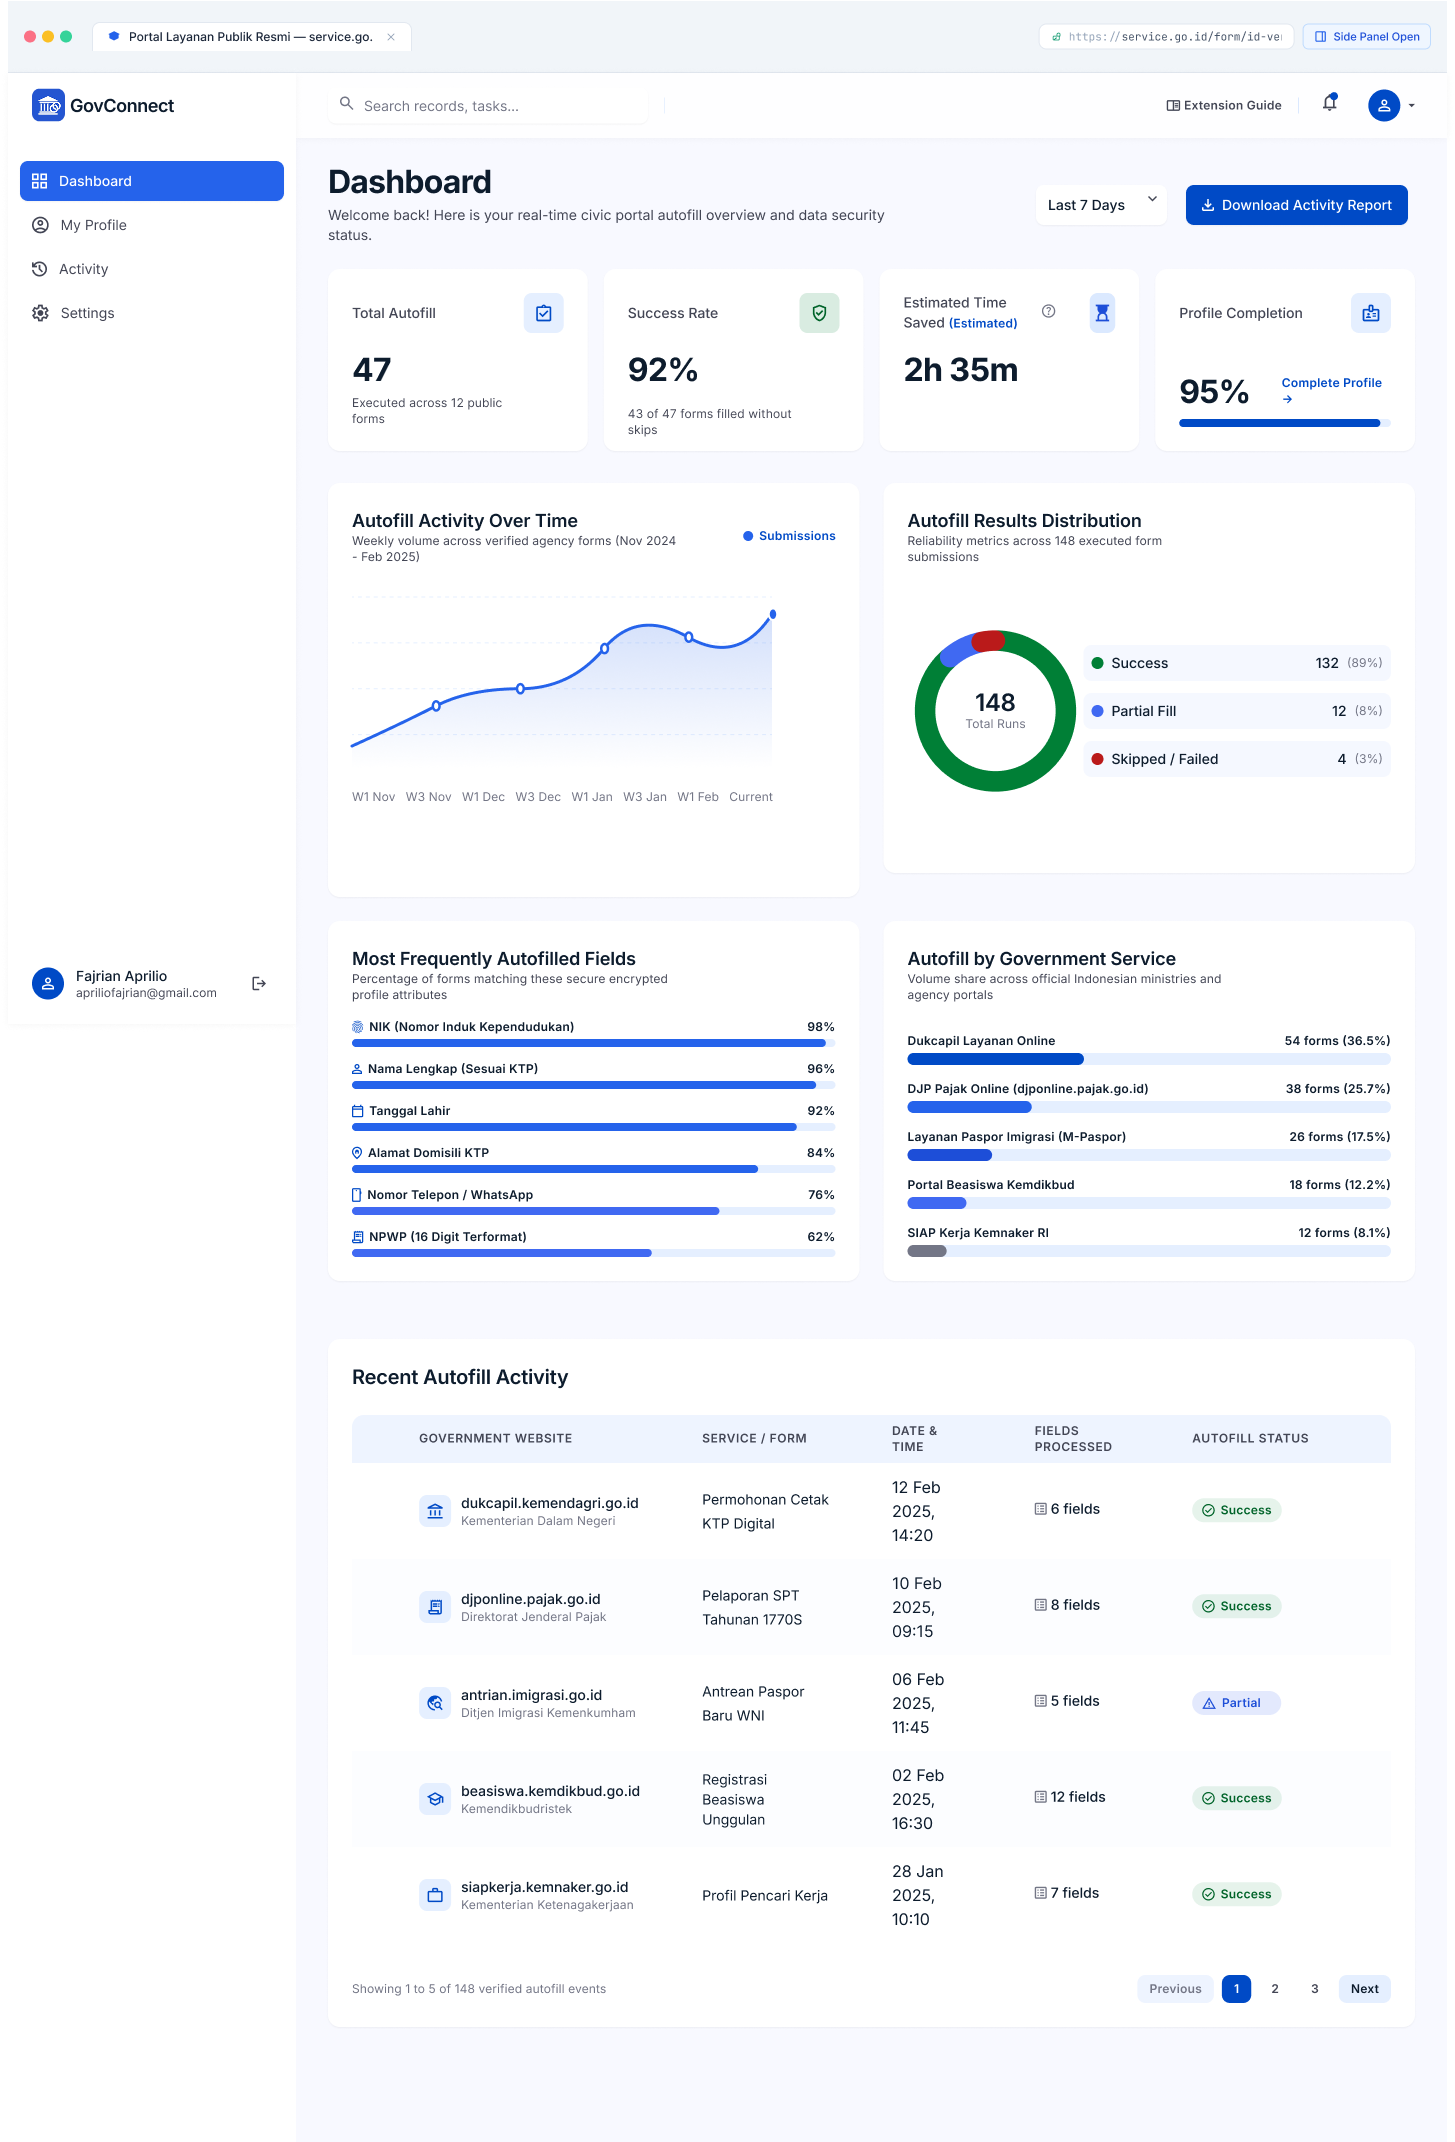
\includegraphics[width=0.65\textwidth, height=0.50\textheight, keepaspectratio]{Main Dashboard.png}
\caption{Antarmuka Halaman Utama (\textit{Main Dashboard}) GovConnect.}
\label{fig:mockup_dashboard}
\end{figure}

\begin{figure}[!ht]
\centering
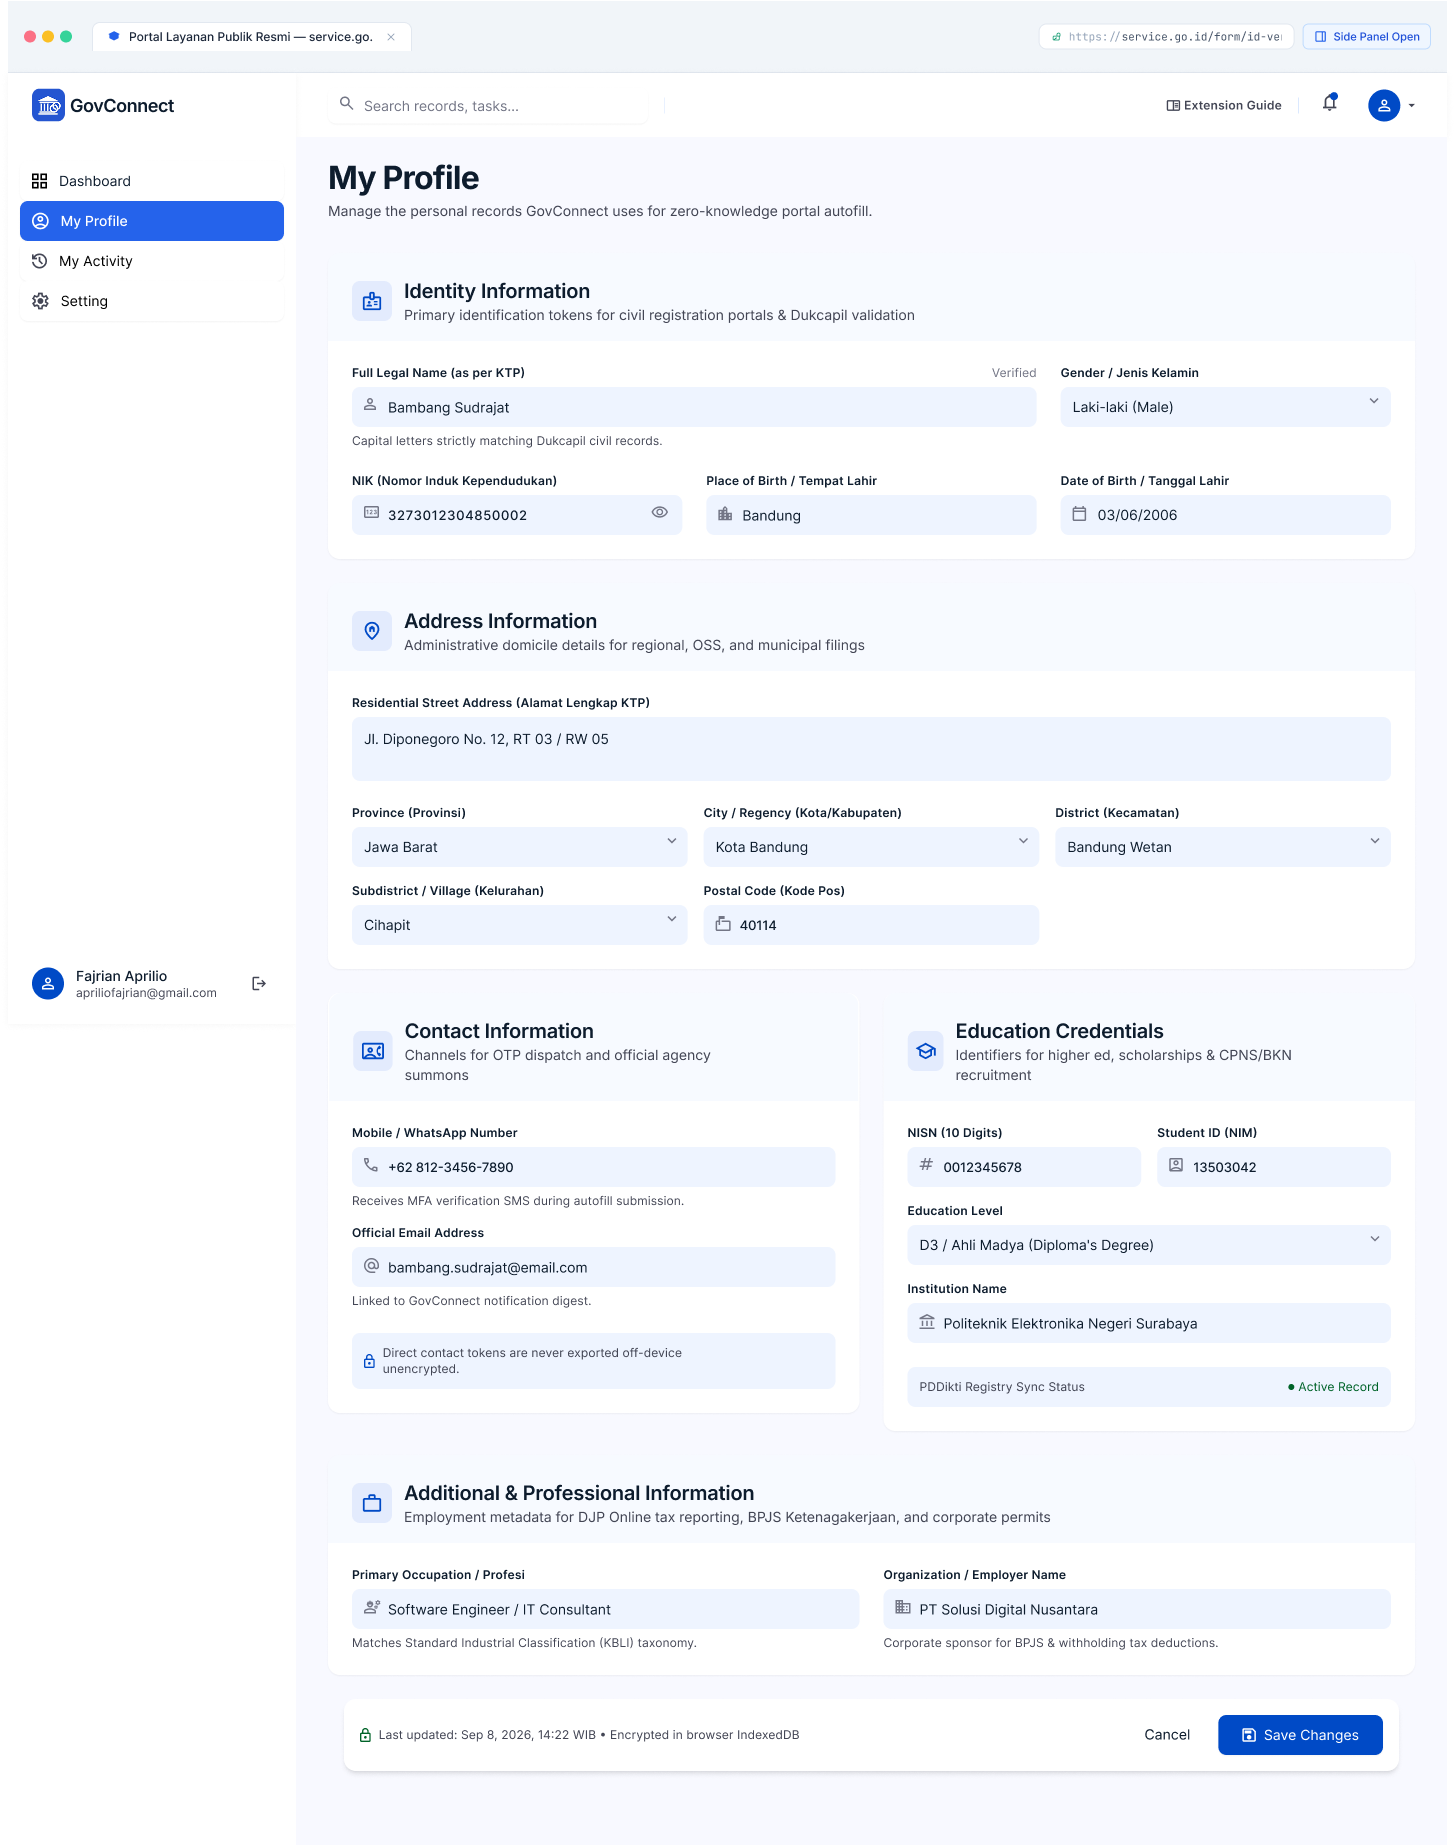
\includegraphics[width=0.65\textwidth, height=0.40\textheight, keepaspectratio]{My Profile.png}
\caption{Halaman Pengelolaan Data Profil Pengguna (\textit{My Profile}).}
\label{fig:mockup_profile}
\end{figure}

\begin{figure}[!ht]
\centering
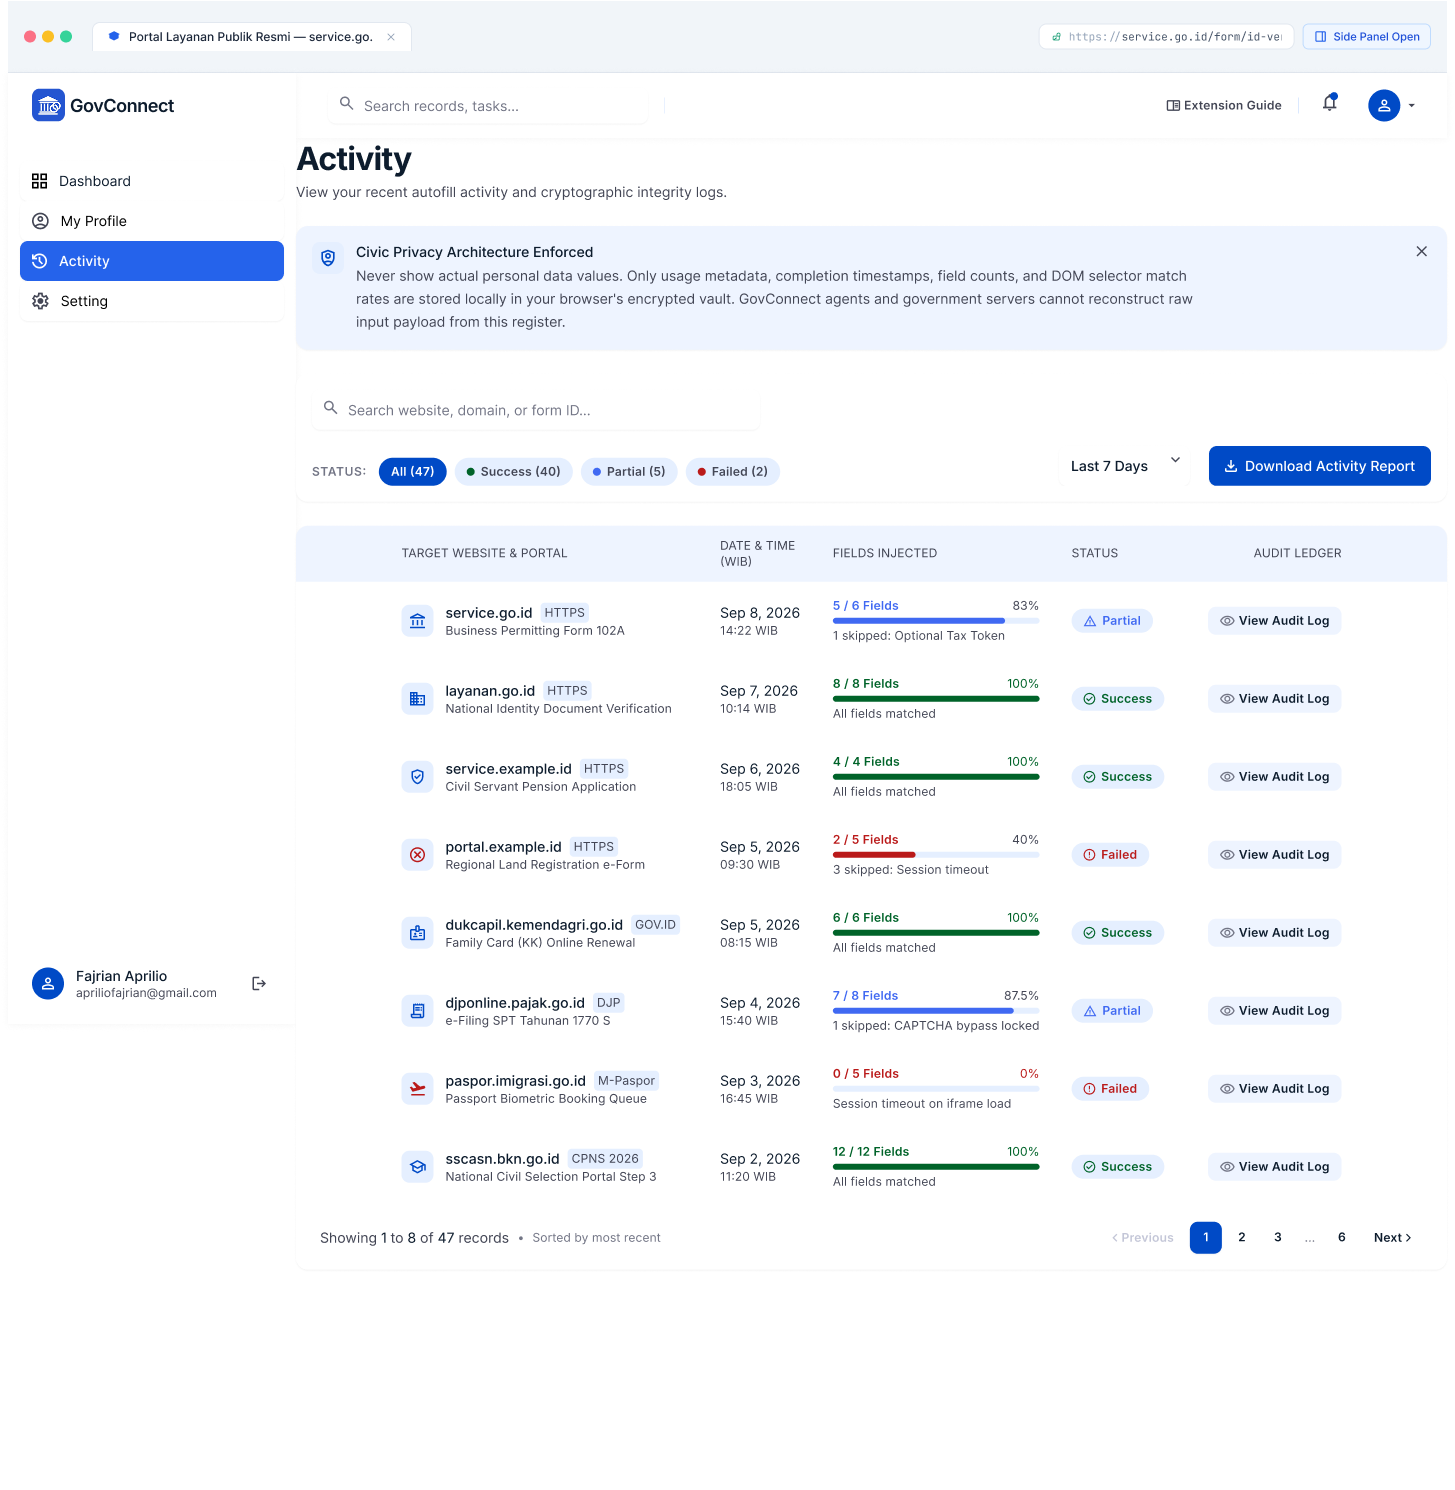
\includegraphics[width=0.65\textwidth, height=0.40\textheight, keepaspectratio]{Activity.png}
\caption{Halaman Riwayat Log Aktivitas Pengisian Formulir (\textit{Activity Log}).}
\label{fig:mockup_activity}
\end{figure}

\begin{figure}[!ht]
\centering
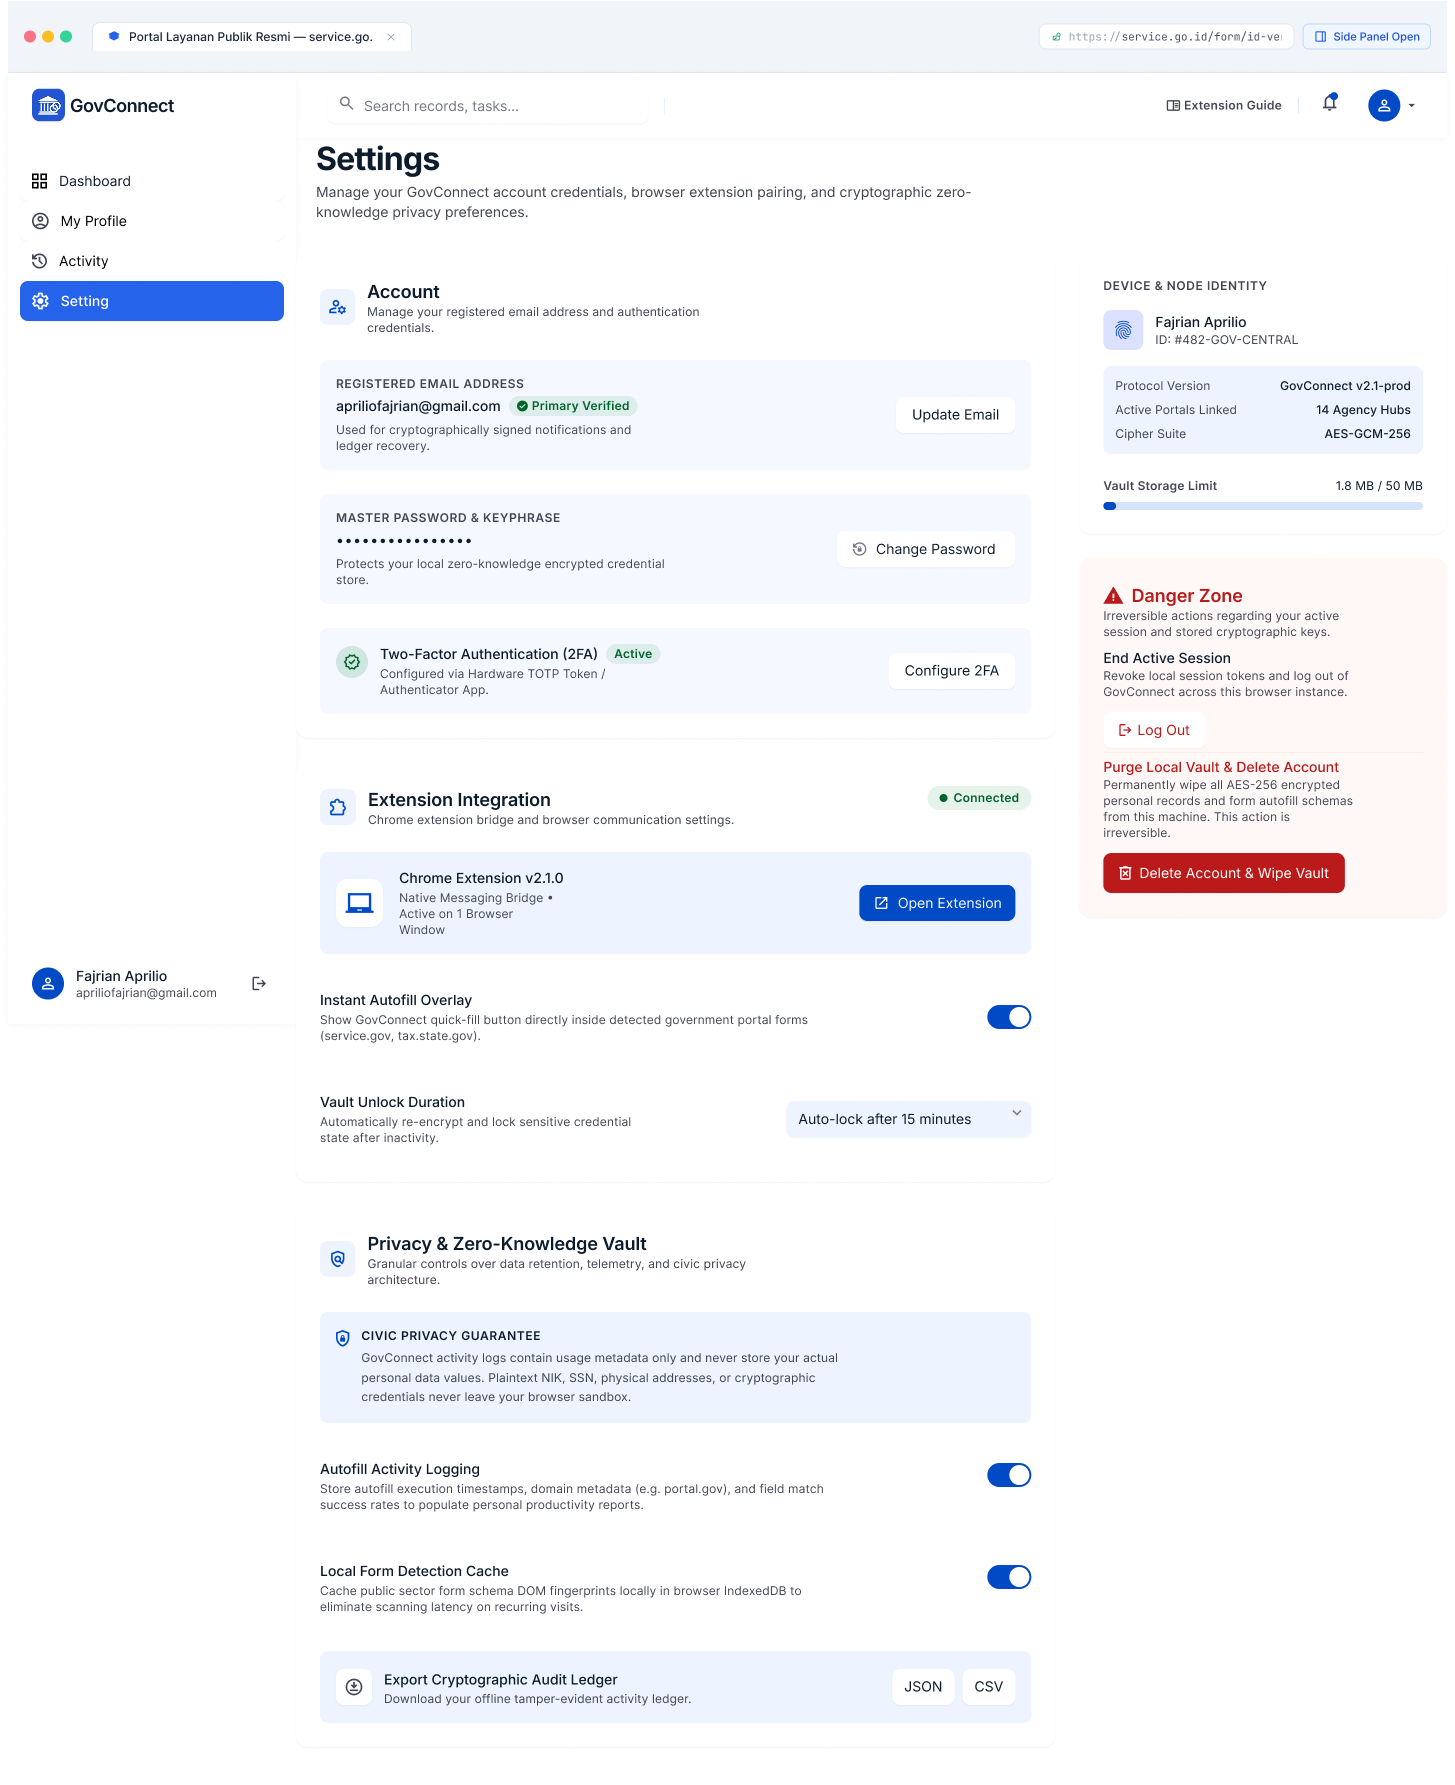
\includegraphics[width=0.65\textwidth, height=0.40\textheight, keepaspectratio]{Setting.png}
\caption{Halaman Pengaturan Akun dan Preferensi Sistem (\textit{Settings}).}
\label{fig:mockup_setting}
\end{figure}

\subsection{Antarmuka Chrome Extension \& Side Panel}
Bagian ekstensi peramban menyajikan interaksi langsung pada situs web target yang mencakup berbagai kondisi operasional:

\begin{figure}[!ht]
\centering
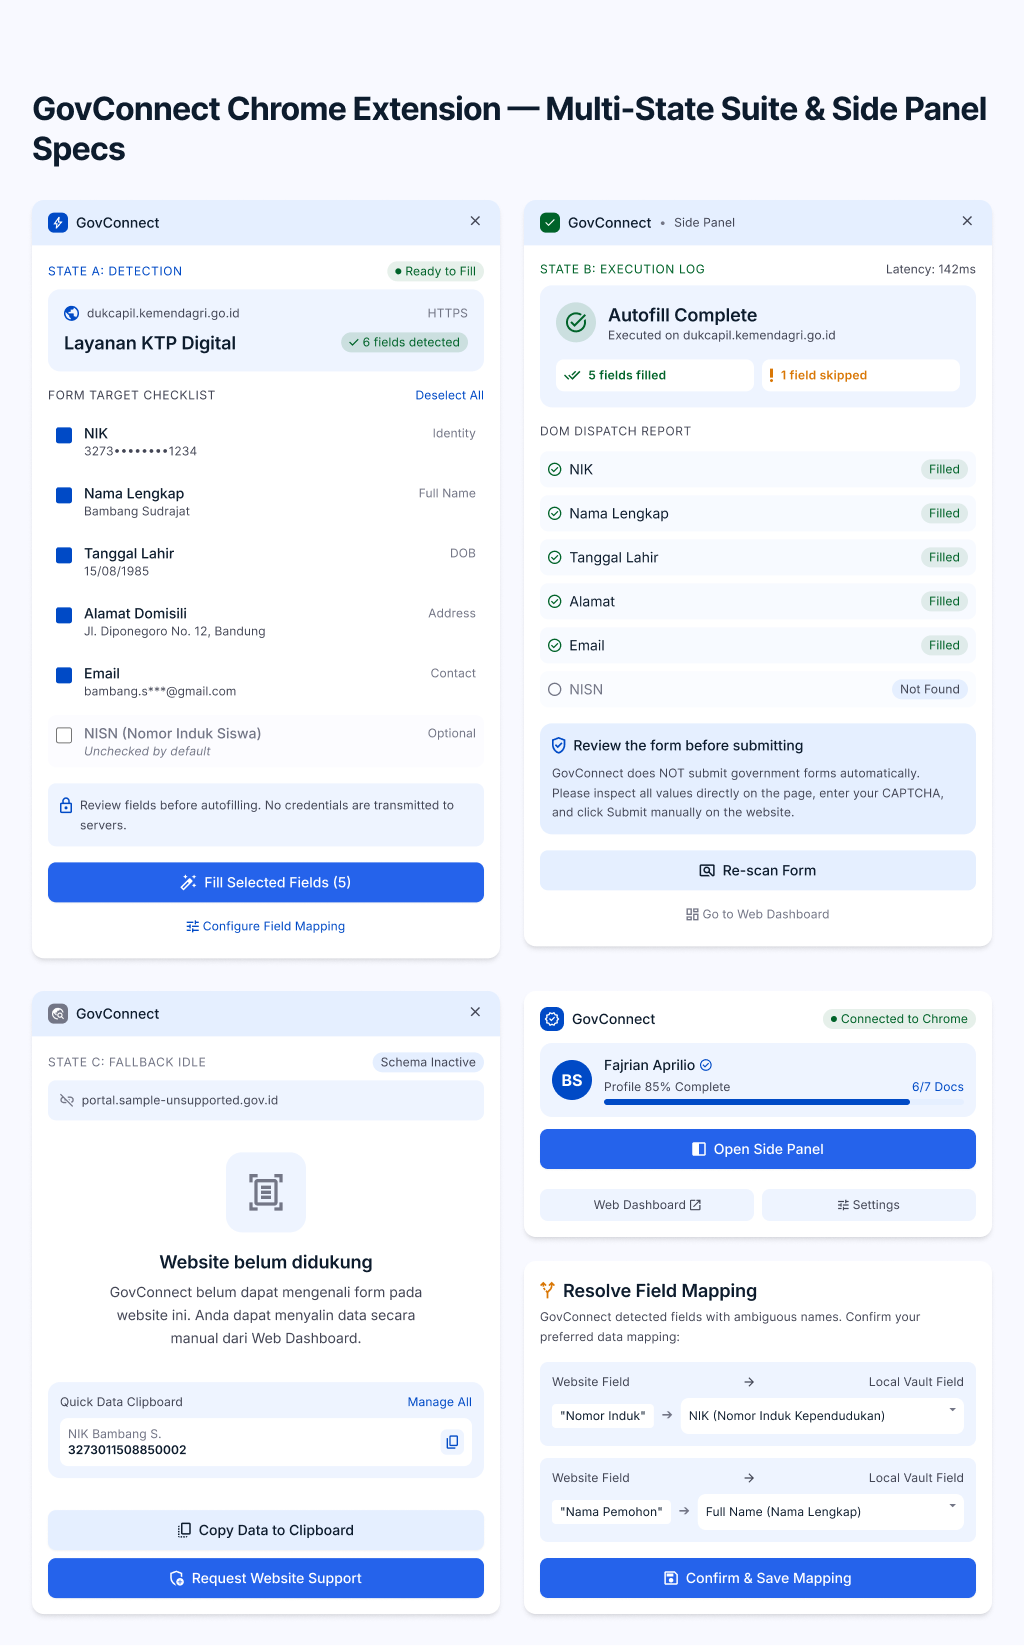
\includegraphics[width=0.45\textwidth, height=0.42\textheight, keepaspectratio]{Frontend Extension.png}
\caption{Tampilan Antarmuka \textit{Popup} Ekstensi Peramban GovConnect.}
\label{fig:mockup_extension}
\end{figure}

\begin{figure}[!ht]
\centering
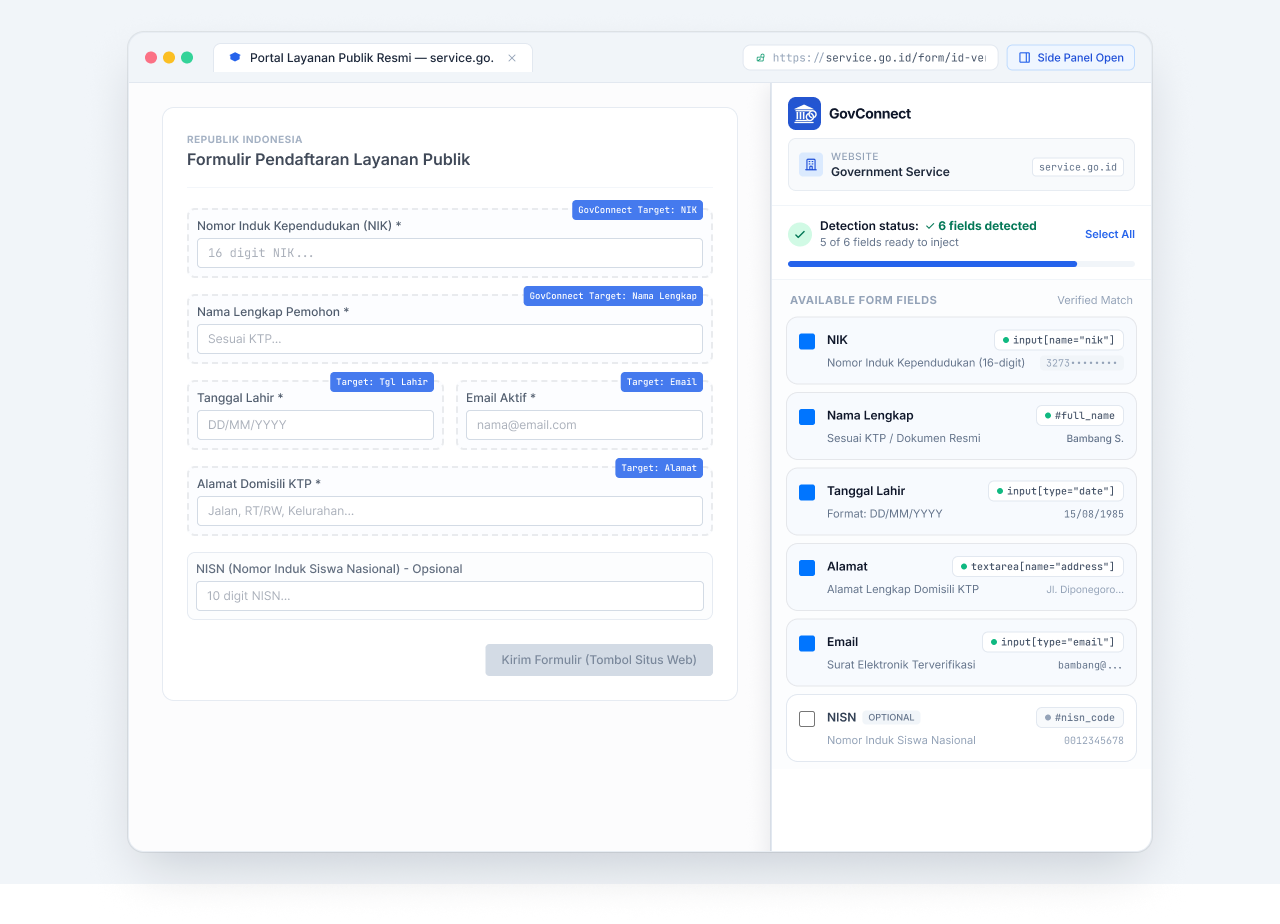
\includegraphics[width=0.65\textwidth, height=0.36\textheight, keepaspectratio]{Side Panel - Form Detected.png}
\caption{\textit{Side Panel}: Status Formulir Terdeteksi (\textit{Form Detected State}).}
\label{fig:mockup_sidepanel_detected}
\end{figure}

\begin{figure}[!ht]
\centering
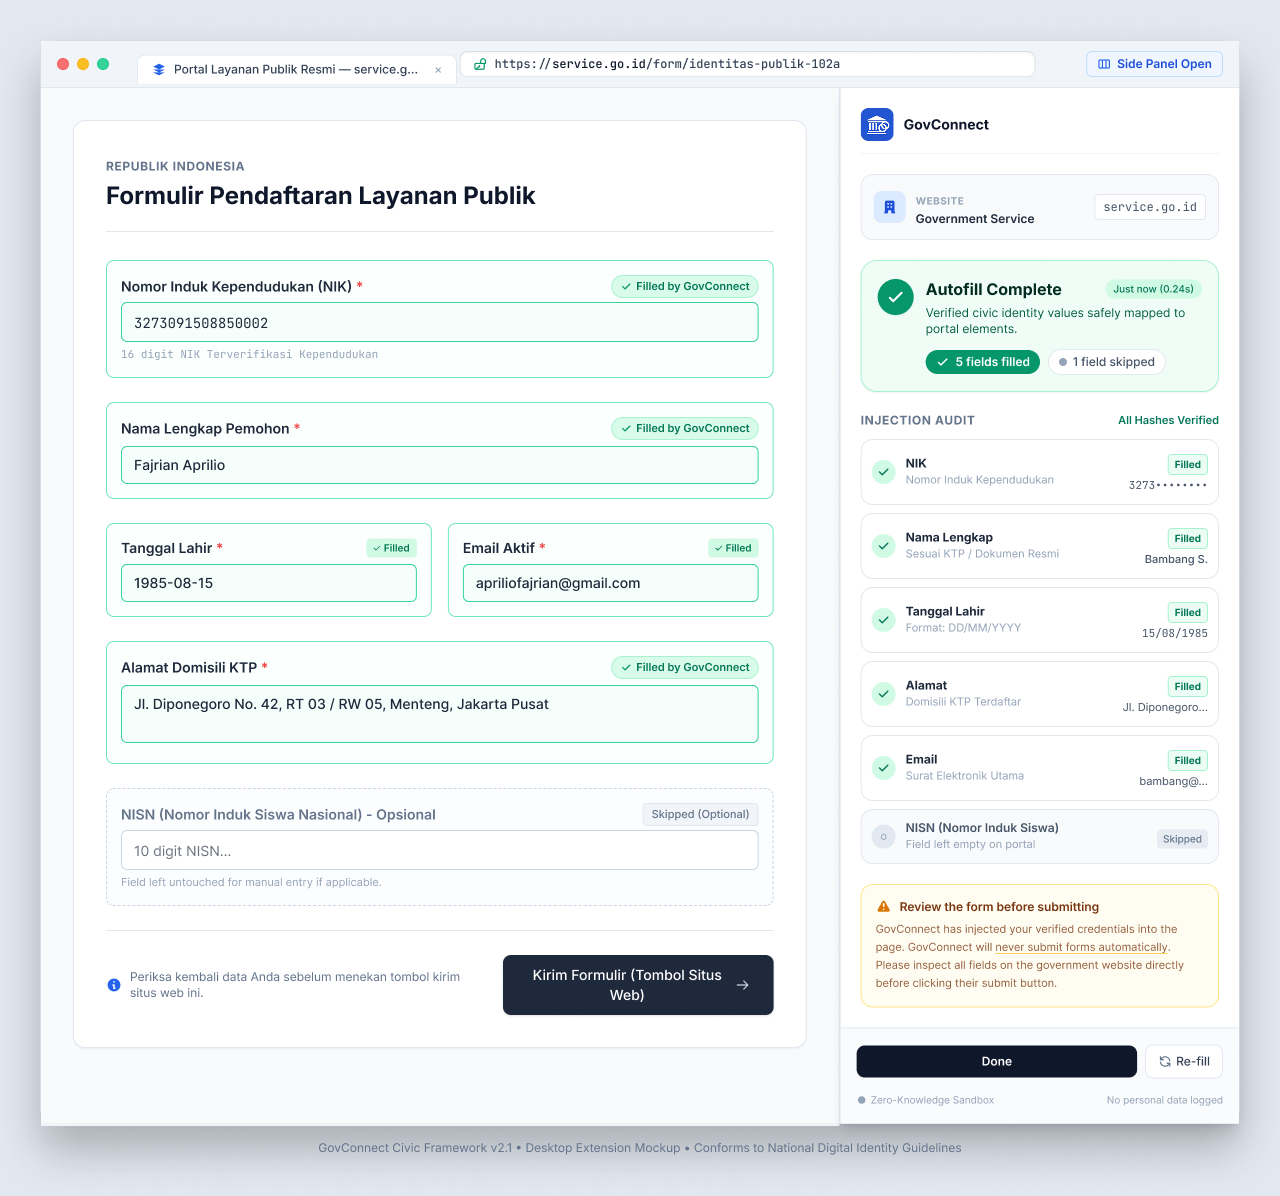
\includegraphics[width=0.65\textwidth, height=0.36\textheight, keepaspectratio]{Side Panel - Autofill Result.png}
\caption{\textit{Side Panel}: Rangkuman Hasil Pengisian (\textit{Autofill Result State}).}
\label{fig:mockup_sidepanel_result}
\end{figure}

\begin{figure}[!ht]
\centering
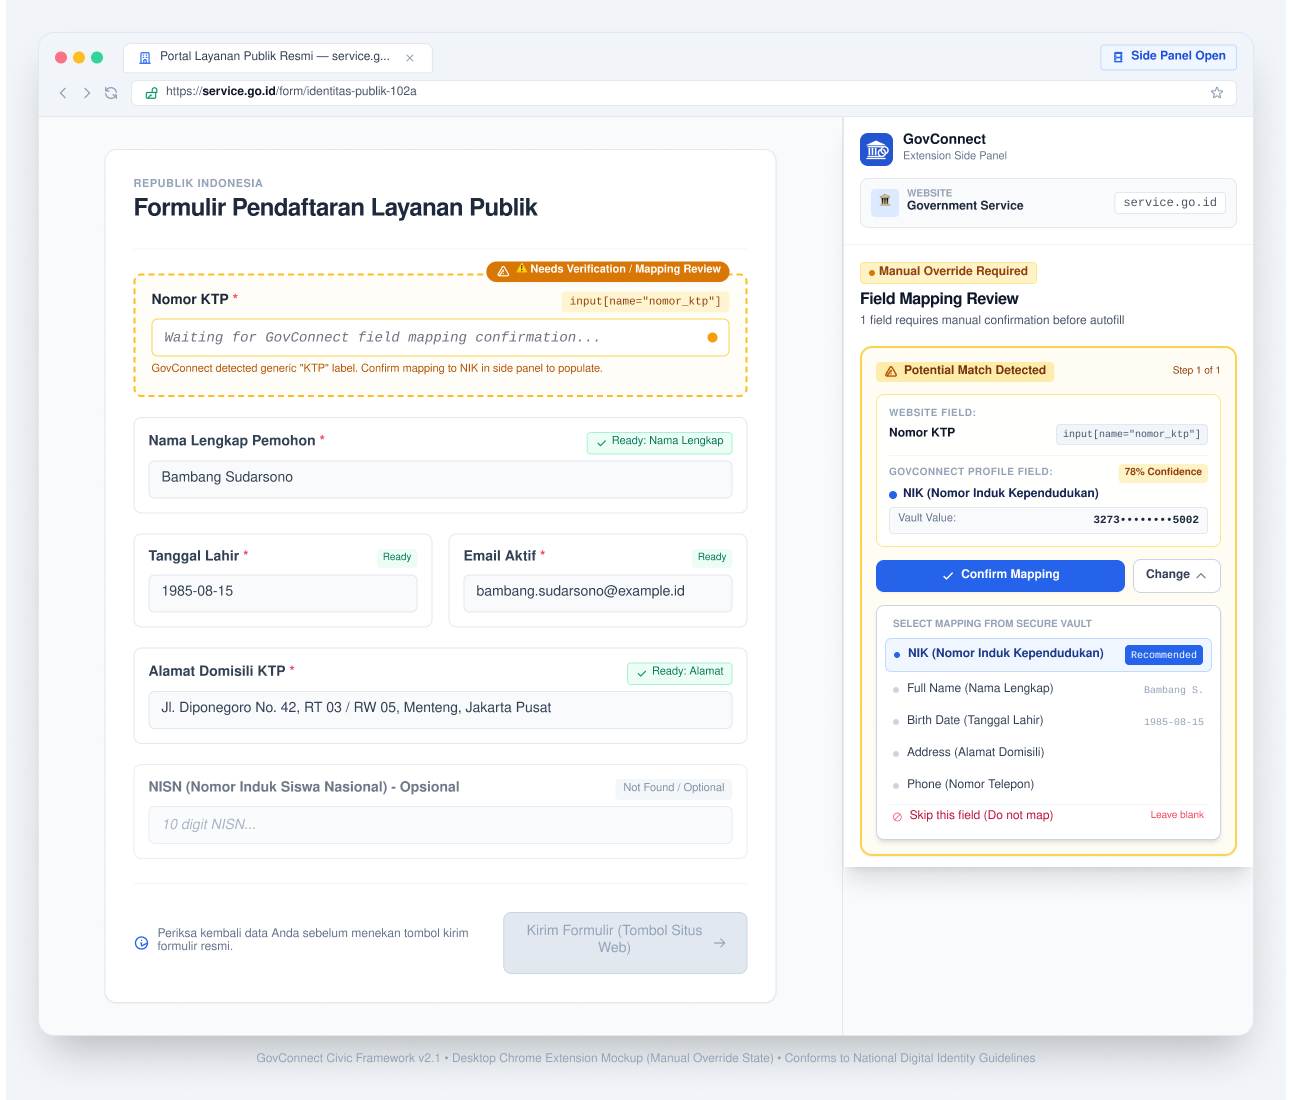
\includegraphics[width=0.65\textwidth, height=0.36\textheight, keepaspectratio]{Side Panel - Manual Override.png}
\caption{\textit{Side Panel}: Pemetaan Manual Field (\textit{Manual Override State}).}
\label{fig:mockup_sidepanel_override}
\end{figure}

\begin{figure}[!ht]
\centering
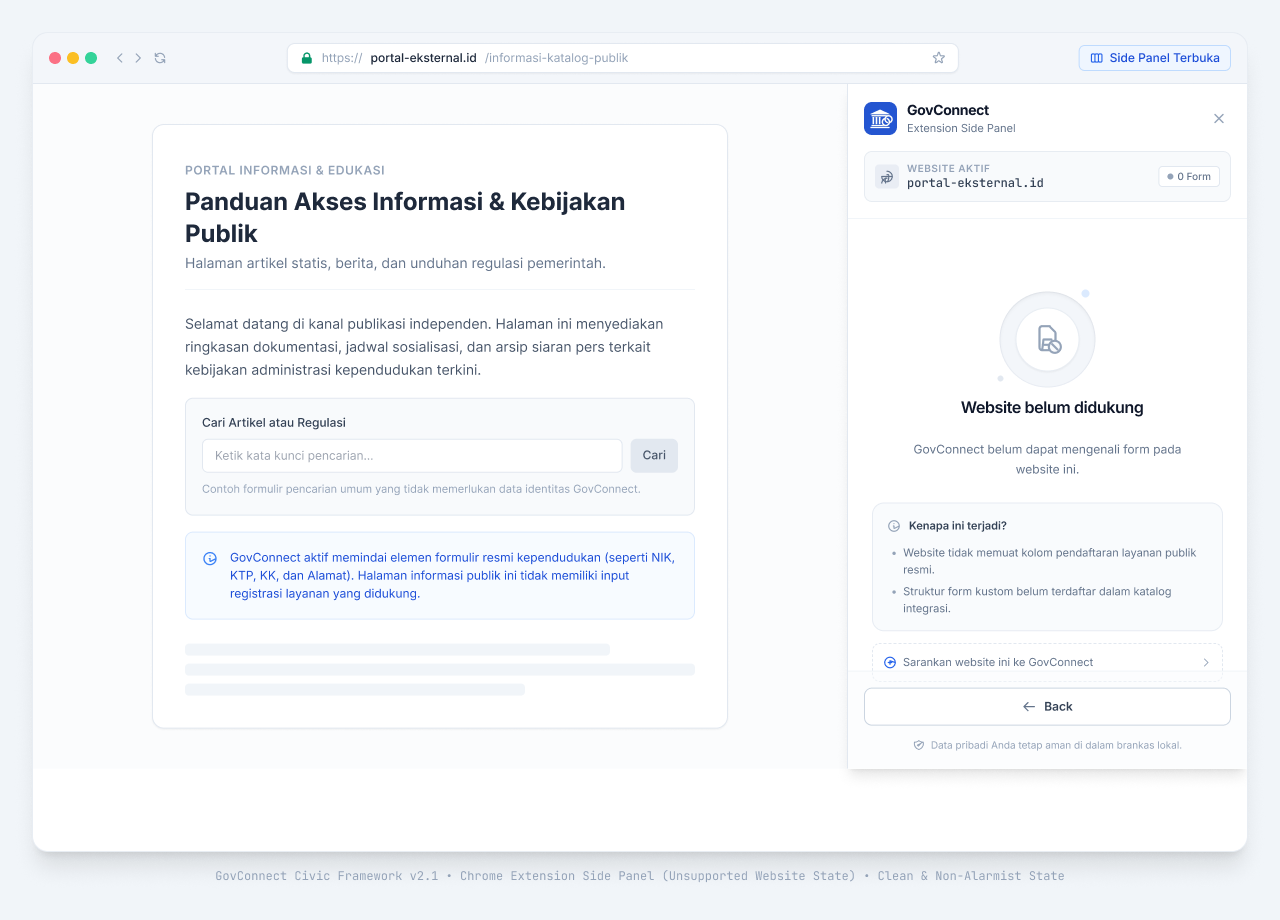
\includegraphics[width=0.65\textwidth, height=0.36\textheight, keepaspectratio]{Side Panel - Unsupported Website.png}
\caption{\textit{Side Panel}: Situs Web Belum Didukung (\textit{Unsupported Website State}).}
\label{fig:mockup_sidepanel_unsupported}
\end{figure}

\end{document}